% !TEX program = xelatex
% =============================================================================
% Block Round --- 授業計画 (ja-JP)
% 高等学校第3学年（高校3年）向け 5授業構成の指導案
% 日本の教育文脈（学習指導要領、共通テスト、JMO/JOI、高専、SSH）に深く適合
% コンパイル: xelatex Plano_de_Aula_ja-JP.tex (TOC生成のため2回実行)
% =============================================================================
\documentclass[12pt,a4paper]{scrartcl}

% ---------- フォントと言語（docs_math/Block_Round_Math_ja-JP と一致）---------
\usepackage{fontspec}
\usepackage{xeCJK}
\setCJKmainfont{Yu Gothic}[Scale=1.05]
\setCJKsansfont{Yu Gothic}[Scale=1.05]
\setmainfont{Latin Modern Roman}[Scale=1.05]
\setsansfont{Latin Modern Sans}[Scale=1.05]
\setmonofont{Latin Modern Mono}
\usepackage{unicode-math}
\setmathfont{Latin Modern Math}[Scale=1.05]

% ---------- パッケージ -------------------------------------------------------
\usepackage{amsmath}
\usepackage{mathtools}

\usepackage[a4paper,top=2.8cm,bottom=2.8cm,left=2.6cm,right=2.6cm,
            headheight=16pt]{geometry}
\usepackage{microtype}
\usepackage{xcolor}
\usepackage{booktabs}
\usepackage{array}
\usepackage{tabularx}
\usepackage{enumitem}
\usepackage{titlesec}
\usepackage{fancyhdr}
\usepackage{graphicx}
\usepackage{csquotes}
\usepackage{tcolorbox}
\tcbuselibrary{skins,breakable}
\usepackage{needspace}
\usepackage{caption}
\usepackage{subcaption}
\usepackage{float}

\raggedbottom

% ---------- Block Round 配色 -------------------------------------------------
\definecolor{accent}{HTML}{5B8E3F}      % マインクラフトの草色
\definecolor{accentdark}{HTML}{406A2A}
\definecolor{earth}{HTML}{825432}        % 土ブロック茶
\definecolor{ink}{HTML}{1F1F23}
\definecolor{muted}{HTML}{4E4E58}
\definecolor{bg}{HTML}{FBF6E9}
\definecolor{rule}{HTML}{D8D1BC}
\definecolor{linkc}{HTML}{2D5A1F}        % リンク用の濃緑

\usepackage[colorlinks=true,
            linkcolor=linkc,
            urlcolor=linkc,
            citecolor=linkc,
            breaklinks=true,
            bookmarks=true,bookmarksopen=true,
            pdftitle={Block Round --- 授業計画 (ja-JP)},
            pdfauthor={Vinicius Rodrigues de Souza}]{hyperref}
\usepackage{xurl}

\color{ink}

\widowpenalty=10000
\clubpenalty=10000

% ---------- 見出しスタイル ---------------------------------------------------
\titleformat{\section}
  {\sffamily\Large\bfseries\color{accent}}{\thesection.}{0.6em}{}
\titleformat{\subsection}
  {\sffamily\large\bfseries\color{accent!85!ink}}{\thesubsection}{0.6em}{}
\titleformat{\subsubsection}
  {\sffamily\normalsize\bfseries\color{muted}}{\thesubsubsection}{0.5em}{}
\titlespacing*{\section}{0pt}{1.2\baselineskip}{0.6\baselineskip}
\titlespacing*{\subsection}{0pt}{0.8\baselineskip}{0.3\baselineskip}
\titlespacing*{\subsubsection}{0pt}{0.6\baselineskip}{0.2\baselineskip}

% ---------- ヘッダ・フッタ ---------------------------------------------------
\pagestyle{fancy}
\fancyhf{}
\fancyhead[L]{\small\sffamily\bfseries\color{accent}BLOCK ROUND}
\fancyhead[R]{\small\sffamily\color{muted}授業計画 --- 高校3年}
\fancyfoot[L]{\small\sffamily\color{muted}Block Round --- 教材}
\fancyfoot[R]{\small\sffamily\color{muted}\thepage 頁}
\renewcommand{\headrulewidth}{0.4pt}
\renewcommand{\footrulewidth}{0.4pt}
\renewcommand{\headrule}{{\color{rule}\hrule height \headrulewidth}}
\renewcommand{\footrule}{{\color{rule}\vskip-\footrulewidth\hrule height \footrulewidth\vskip-\footrulewidth}}

% ---------- 教育用ボックス（環境名はASCII、表示題はJP）----------------------
\newtcolorbox{shiki}{
  colback=bg, colframe=rule, boxrule=0.4pt, arc=2pt,
  left=10pt,right=10pt,top=8pt,bottom=8pt,
  before skip=8pt, after skip=8pt,
  fontupper=\color{accentdark}, breakable,
  before={\par\needspace{4\baselineskip}}
}

\newtcolorbox{katsudou}[1][活動]{
  enhanced, breakable,
  colback=bg, colframe=accent, boxrule=0.6pt, arc=4pt,
  left=12pt,right=12pt,top=10pt,bottom=10pt,
  before skip=12pt, after skip=12pt,
  before={\par\needspace{5\baselineskip}},
  attach boxed title to top left={xshift=10pt,yshift=-8pt},
  boxed title style={colback=accent,colframe=accent,boxrule=0pt,arc=2pt},
  coltitle=white, fonttitle=\sffamily\bfseries\small,
  title=#1
}

\newtcolorbox{memo}[1][指導上の留意点]{
  enhanced, breakable,
  colback=bg!50!white, colframe=rule, boxrule=0.4pt, arc=2pt,
  left=10pt,right=10pt,top=8pt,bottom=8pt,
  before skip=8pt, after skip=8pt,
  before={\par\needspace{3\baselineskip}},
  attach boxed title to top left={xshift=10pt,yshift=-7pt},
  boxed title style={colback=muted,colframe=muted,boxrule=0pt,arc=2pt},
  coltitle=white, fonttitle=\sffamily\bfseries\footnotesize,
  title=#1
}

\newtcolorbox{shidou}[1][学習指導要領]{
  enhanced,
  breakable=false,
  colback=bg!70!white, colframe=accent!60!ink, boxrule=0.4pt, arc=2pt,
  left=10pt,right=10pt,top=6pt,bottom=6pt,
  before skip=6pt, after skip=6pt,
  before={\par\needspace{8\baselineskip}},
  attach boxed title to top left={xshift=10pt,yshift=-6pt},
  boxed title style={colback=accent!60!ink,colframe=accent!60!ink,boxrule=0pt,arc=2pt},
  coltitle=white, fonttitle=\sffamily\bfseries\footnotesize,
  title=#1
}

\newtcolorbox{minecraft}[1][マインクラフト]{
  enhanced, breakable,
  colback=accent!7, colframe=earth!70!accent, boxrule=0.5pt, arc=3pt,
  left=10pt,right=10pt,top=8pt,bottom=8pt,
  before skip=10pt, after skip=10pt,
  before={\par\needspace{3\baselineskip}},
  attach boxed title to top left={xshift=10pt,yshift=-7pt},
  boxed title style={colback=earth,colframe=earth,boxrule=0pt,arc=2pt},
  coltitle=white, fonttitle=\sffamily\bfseries\footnotesize,
  title=#1
}

\setlength{\parskip}{0.75em}
\setlength{\parindent}{0pt}
\linespread{1.10}

\setlength{\textfloatsep}{14pt plus 2pt minus 2pt}
\setlength{\floatsep}{14pt plus 2pt minus 2pt}
\setlength{\intextsep}{14pt plus 2pt minus 2pt}

\captionsetup{font=small, labelfont={bf,color=accent}, textfont={color=muted}, justification=centering}
\captionsetup[sub]{font=footnotesize, labelfont={bf,color=accent!75!ink}, textfont={color=muted}}

\graphicspath{{img/}}

\newcommand{\code}[1]{\texttt{\small #1}}
\newcommand{\acc}[1]{\textcolor{accent}{\textbf{#1}}}
\newcommand{\cmd}[1]{\textcolor{earth}{\texttt{\small #1}}}
\newcommand{\tempo}[1]{\textnormal{\footnotesize\color{bg!90!white}\textsf{#1}}}

\begin{document}

% =============================================================================
% 表紙
% =============================================================================
\begin{titlepage}
  \centering
  \vspace*{3.0cm}
  {\sffamily\bfseries\fontsize{56}{60}\selectfont \color{accent} Block Round\par}
  \vspace{0.7cm}
  {\sffamily\LARGE\color{muted} 授業計画\par}
  \vspace{0.25cm}
  {\sffamily\Large\color{muted} 高等学校第3学年（高校3年）\par}
  \vspace{1.0cm}
  {\color{rule}\rule{0.6\textwidth}{0.6pt}\par}
  \vspace{0.7cm}
  \begin{minipage}{0.84\textwidth}
    \centering\color{ink}\large
    本書は、ボクセル生成ツール\emph{Block Round}を活用し、日本の高校3年生を対象とした
    全5回（各50分）の数学指導案である。\emph{解析幾何}・\emph{計算論的思考}・
    \emph{デジタル・シティズンシップ}・そして世界で最も普及した\emph{マインクラフト}
    での建築実践を、ひとつの問いの周囲に統合する。すなわち、
    \emph{連続的な曲線を有限のボクセル格子の上にどう表すか、そしてその表現を、
    現代の高校生が最も親しむ仮想世界の建造可能な構造物にどう翻訳するか}。
  \end{minipage}
  \vspace{0.7cm}\\
  {\color{rule}\rule{0.6\textwidth}{0.6pt}\par}
  \vspace{0.9cm}
  \begin{minipage}{0.78\textwidth}
    \centering
    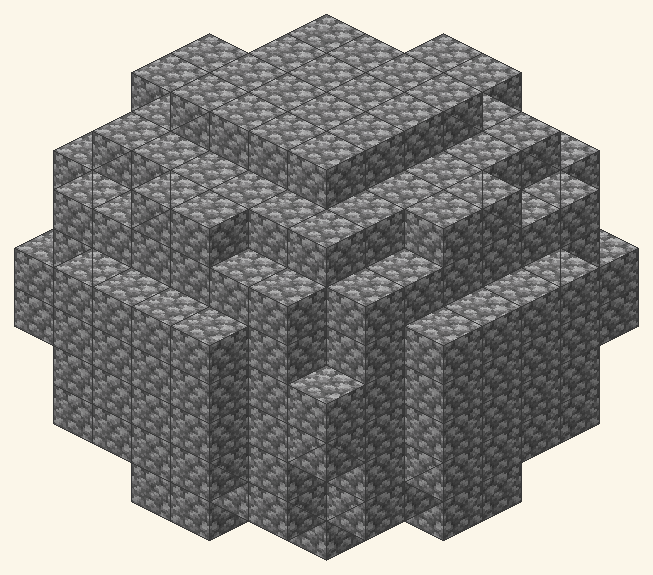
\includegraphics[width=0.55\linewidth]{fig10_3d_sphere_d12.png}\\[0.4em]
    {\sffamily\footnotesize\color{muted}Block Roundによって直径10にボクセル化された球を、
    マインクラフトの\emph{cobblestone}（丸石）テクスチャで描画したもの。}
  \end{minipage}
  \vspace{0.7cm}\\
  {\color{rule}\rule{0.6\textwidth}{0.6pt}\par}
  \vspace{0.9cm}
  \begin{minipage}{0.82\textwidth}
    \centering\sffamily\small\color{muted}
    \textbf{関連教科：}数学 $\cdot$ 国語・芸術（デジタルアート・デザイン） $\cdot$ 情報 $\cdot$ デジタル・シティズンシップ $\cdot$ ゲーム教育 \\[0.4em]
    \textbf{適合：}高等学校学習指導要領（平成30年告示・令和4年実施） $\cdot$ 大学入学共通テスト数学・情報 $\cdot$ \hyperref[sec:jmo]{JMO/JOI} $\cdot$ マインクラフト教育版（Minecraft Education）
  \end{minipage}
\end{titlepage}

% =============================================================================
\renewcommand{\contentsname}{\color{accent}目次}
\tableofcontents
\thispagestyle{fancy}
\newpage

% =============================================================================
\section{単元の位置づけと背景}\label{sec:identificacao}

\begin{center}
\begin{tabular}{@{}p{0.32\textwidth}p{0.62\textwidth}@{}}
\toprule
\textbf{教科} & 数学（芸術・情報・工学・歴史・地理との強い教科横断的接続を持つ）。 \\
\addlinespace[2pt]
\textbf{学校段階・学年} & 高等学校第3学年。第2学年および定時制・通信制への適応も可能。国公立・私立、普通科・専門学科のいずれにも対応する。 \\
\addlinespace[2pt]
\textbf{対象課程} & 全日制（昼間）、定時制、通信制、総合学科、工業高校・商業高校・農業高校等の専門学科、高等専門学校（高専、5年制の本科3年次に相当）。 \\
\addlinespace[2pt]
\textbf{総時数} & 50分授業×5回（教室で250分）+ 任意の課外活動。100分連続授業×2.5回への変換例は §\ref{sec:adapt} に記載。 \\
\addlinespace[2pt]
\textbf{中核教材} & Block Round --- 無料のWebアプリケーション。登録不要、サーバー不要、初回読み込み後はオフライン動作（PWA）。個人情報保護法（APPI）に準拠し、個人データを収集・送信しない。低価格スマートフォンでも動作し、Javaやマインクラフト本体のインストールを要求しない。 \\
\addlinespace[2pt]
\textbf{学習指導要領との関連} & 「図形と方程式」「数列・ベクトル」「立体図形」「平面上の曲線」「複素数平面」（数学I・II・III、数学A・B・C） $\cdot$ 数学的活動 $\cdot$ 数学的な見方・考え方の育成 $\cdot$ 情報科（情報I）の問題解決とアルゴリズム。 \\
\addlinespace[2pt]
\textbf{進路・キャリア接続} & 大学入学共通テスト数学・情報の対策、個別大学2次試験対応、推薦型・総合型選抜のポートフォリオ素材、SSH指定校の課題研究テーマ、高専・専門学科の課題制作。 \\
\addlinespace[2pt]
\textbf{関連コンテスト・大会} & \hyperref[sec:jmo]{日本数学オリンピック (JMO)}、日本ジュニア数学オリンピック (JJMO)、数学甲子園、日本情報オリンピック (JOI)、パソコン甲子園、U-22プログラミング・コンテスト、スーパーサイエンスハイスクール (SSH) 成果発表会、マインクラフトカップ全国大会。 \\
\addlinespace[2pt]
\textbf{既習事項} & 平面上の座標（数学I・II「図形と方程式」）、円の方程式、基本図形の面積と体積（数学I・A・B）、関数の概念、比例と百分率。マインクラフトへの親しみ（推奨だが必須ではない。Block Round 自体はゲームを必要としない）。 \\
\addlinespace[2pt]
\textbf{教員の事前準備} & Block Round の予備操作（20分）、技術解説書『\texttt{docs\_math/Block\_Round\_Math\_ja-JP.pdf}』の通読、可能であればマインクラフト Java版のコマンド \cmd{/fill}、\cmd{/clone}、\cmd{//sphere} の概要把握。 \\
\bottomrule
\end{tabular}
\end{center}

\begin{memo}[日本の高校の多様性に対応する設計]
本指導案は、日本の高校3年の多様な現場で実施可能になるよう設計されている。すなわち、東京・横浜・大阪・名古屋・福岡などの都市部の公立進学校と、中高一貫校（麻布・武蔵・桜蔭・女子学院など）と、地方の県立公立高校と、工業・商業・農業・水産・福祉などの専門学科と、高等専門学校（高専、国立53校・公立3校・私立3校）と、北海道・東北・九州・沖縄の離島・過疎地高校と、アイヌ民族や在日コリアン・新興留学生（ブラジル人学校 — 浜松・豊橋・群馬太田）を多く含む学校と、定時制・通信制と、高等専修学校と、スーパーサイエンスハイスクール（SSH）指定校（文部科学省指定、約220校）まで。それぞれに固有の調整を §\ref{sec:adapt} に整理した。Block Round が採用された理由はまさにここにある。\emph{すべての現場で動く}からだ。低価格スマホでも、初回読み込み後はオフラインでも、登録なしでも、個人データを送信しないので個人情報保護法（APPI）・GIGAスクール構想の指針にも適合する。
\end{memo}

\begin{minecraft}[本指導案がマインクラフトを軸とする理由]
マインクラフトは史上最も売れたゲーム（3億本超）であり、日本でもニコニコ動画での実況文化（2011年頃〜）以降、世代を超えた文化的参照点となっている。ヒカキン（HikakinTV）、まいぜんシスターズ（子ども向け）、赤髪のとも、カズクラ、兄者弟者（2BRO）など、複数の人気YouTuber/配信者がマインクラフトを継続的に取り上げ、視聴者層は中学生から高校生・大学生まで広い。\emph{マインクラフトカップ全国大会}は文部科学省後援の公式コンテストとして毎年開催され、SDGs等のテーマで全国の小中高生・高専生・特別支援学校生が建築作品を競う。本指導案でマインクラフトを軸に据えるのは流行への迎合ではなく、\emph{日本の高校生がすでに生きていて、すでに幾何学をしている場所を認めること}に他ならない。
\end{minecraft}

% =============================================================================
\section{教育的根拠}\label{sec:justificativa}

Block Roundを高校3年の指導教材として選ぶ理由は、日本の現代教育が抱える\acc{五つの要請}に同時に応えることにある。第一に、形式的な数学と情報リテラシーの統合（学習指導要領「情報I」必修化・令和4年度実施、「情報II」令和5年度開講、令和7年度共通テスト「情報」導入と直接連動する）。第二に、抽象的知識を、生徒にとって意味のある実践のなかで文脈化すること（数学的活動・「数学的な見方・考え方」育成の柱）。第三に、共通テスト・個別大学2次試験で頻出の「図形と方程式」「立体図形」「数列」「ベクトル」「平面上の曲線」分野への準備。第四に、新しい学習指導要領が掲げる「探究的な学び」「主体的・対話的で深い学び」「STEAM教育」の三本柱との接続。第五に、世界的に最も普及している若者文化のひとつ\emph{マインクラフト}を、数学的厳密性を失わずに動機づけの橋とすることである。

\emph{ボクセル・アート}は今日の日本の若者文化において中心的な位置を占めている。マインクラフトは2009年に Markus Persson（スウェーデン）によって誕生し、2014年に Microsoft が25億米ドルで買収、現在はマインクラフト教育版（Minecraft Education）として世界の学校に展開されている。日本では、文部科学省「教育の情報化」推進事業の一環として、東京都・大阪府・神奈川県の一部自治体や私立学校で導入が進む。ボクセル建築を出発点とすることは、生徒にとって親しい\emph{遊び}の伝統を、\emph{真正の数学問題}へ転換する操作にほかならない。すなわち「$1\times1\times1$ のブロック離散格子の上に、$\mathbb{R}^3$ 上で解析的に定義された形をいかに記述するか」である。サーバーで毎日のように立方体・塔・農場・ドームを造っている生徒は、自分が直感で行ってきたことに正式な名前があったことを発見する。\emph{ボクセル化}、\emph{離散ラスタライゼーション}、\emph{楕円体の陰関数方程式}。

この教育的転換は、日本の教育思想の五つの伝統と対話する。

\begin{itemize}[leftmargin=1.3em,itemsep=0.2em,topsep=0.3em]
  \item \acc{福沢諭吉}（1835--1901、慶應義塾創設者、『学問のすゝめ』1872--1876）。生徒の身近な文化（マインクラフト・スマホ・YouTube）からこそ「実学」の出発点を設定するという姿勢は、福沢の「実学」観に通じる。Block Round は\emph{形式偏重}を排し、目の前のスクリーンで\emph{結果が確かめられる}知をめざす。

  \item \acc{遠山啓}（1909--1979）と\acc{数学教育協議会（AMI）}による\emph{水道方式}。算数・数学の概念を一意な「水路」として可視化するこの方法論は、Block Round 的アプローチ（同じ円を三つの「水路」＝アルゴリズムが流す）に最も近い日本の伝統である。遠山の\emph{量の体系}（外延量と内包量、複合量）は、ボクセル数とブロック容量（外延量）、密度とテクスチャ（内包量）、所要時間と効率（複合量）として本指導案にそのまま再現されている。継承者の\acc{銀林浩}（『量の世界の発見』）も同様。

  \item \acc{大村はま}（1906--2005、国語教育の革命家、単元学習）。「生徒個別の能力に合わせた指導」と「単元としての一貫した問題解決」は、本指導案の5授業の連続的構成（同じ問題＝ボクセル化を、5段階で深化する）の設計原理にあたる。

  \item \acc{倉橋惣三}（1882--1955、東京女子高等師範学校）の「生活即教育」、すなわち学習は生活の延長から始まるという立場。マインクラフトをやっている高校生にとって、ボクセル化はすでに「生活」の一部である。

  \item \acc{民族数学（エスノマスマティクス）}の伝統。ブラジルの \acc{ウビラタン・ダンブロジオ}（1932--2021、ICMI Felix Klein 賞2005）が体系化したこの研究領域は、日本でも横地清・横山悦郎らによって紹介されてきた。Block Round の三つのアルゴリズム（ユークリッド、ブレゼンハム、閾値）は、同じ問題に対する三つの民族数学的応答として読むことができる。さらに、日本のマインクラフト共同体が YouTube で日本語の構築チュートリアルを介して伝承する建築知も、\emph{第四の民族数学}（口頭で・ゲームを介して・現代的に媒介された）にほかならない。

\end{itemize}

ソフトウェアの存在は明確な認識論的機能を果たす。代数を\emph{代替する}のではなく、互いに競合する数学的定式化の\emph{差異を可視化する}。三つのアルゴリズムは、同一の対象（離散円）に対する三つの数学的に異なる定義であり、Figure~\ref{fig:comp-d10} のように目視できる別個の絵を生む。生徒は\emph{目で}「定義が結果を決める」ことを学び、同時にその結果は抽象ではないことも学ぶ。\emph{まさにそれを、マインクラフトで一個一個のブロックとして組み立てられる}のである。

\begin{figure}[!htbp]
\centering
\begin{subfigure}[t]{0.31\linewidth}\centering
  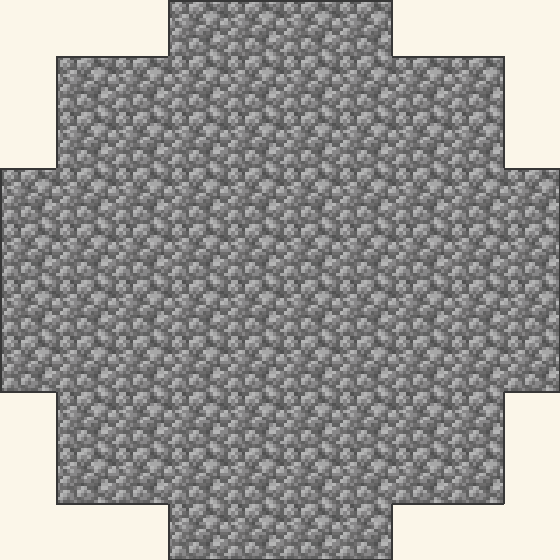
\includegraphics[width=\linewidth]{fig01_2d_d10_euclidean.png}
  \caption{\emph{ユークリッド}}
\end{subfigure}\hfill
\begin{subfigure}[t]{0.31\linewidth}\centering
  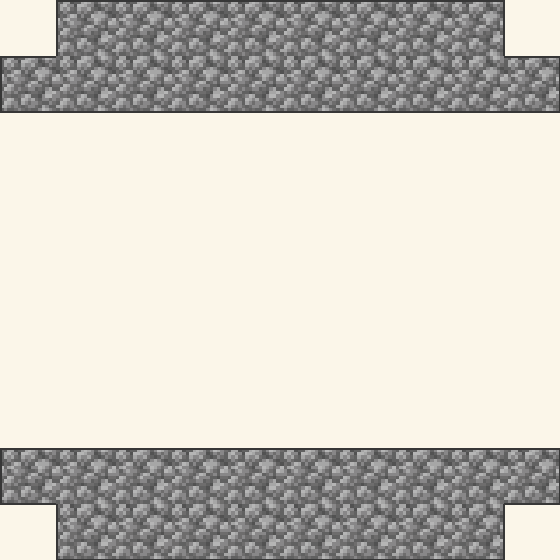
\includegraphics[width=\linewidth]{fig02_2d_d10_bresenham.png}
  \caption{\emph{ブレゼンハム}}
\end{subfigure}\hfill
\begin{subfigure}[t]{0.31\linewidth}\centering
  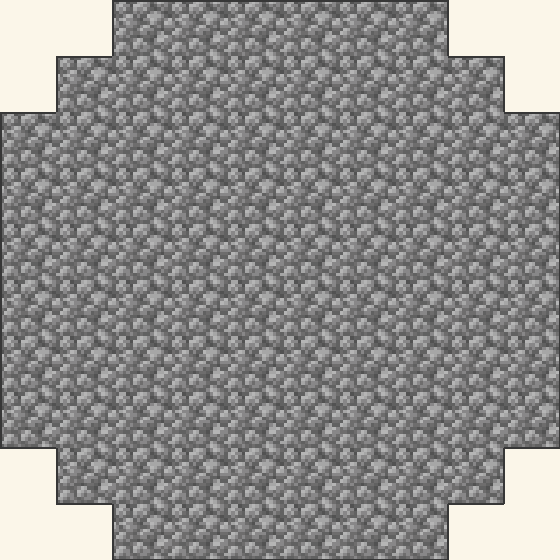
\includegraphics[width=\linewidth]{fig03_2d_d10_threshold.png}
  \caption{\emph{閾値}}
\end{subfigure}
\caption{同じ直径10の円を三つの判定基準で描いたもの。マインクラフトの\emph{cobblestone}（丸石）テクスチャで描画。隅のセル、行間の遷移、東西南北の頂点の扱いがそれぞれ異なる。これらは三つの\emph{数学的に正しい}答えであり、マインクラフトでの三つの異なる建築設計図でもある。}
\label{fig:comp-d10}
\end{figure}

\begin{memo}[公正性と日本の高校現場の物的現実]
Block Round の選定は、教材の物的アクセス公正性に対する具体的な配慮でもある。文部科学省「GIGAスクール構想」（2019年〜）により小中学生には1人1台端末が配備されたが、高校段階では自治体ごとの差が大きい。BYOD（生徒所有端末の活用）が前提となる学校もあれば、教室の共用端末を使う学校もある。一方、高校生のスマートフォン所有率は95\%超（総務省「情報通信白書」、内閣府「青少年のインターネット利用環境実態調査」）と極めて高い。Block Round はまさにこの実状を念頭に設計されている。低価格スマホ、常時インターネット接続不要、登録・ログイン不要。さらに付録~\ref{ap:adapt-analog} に\emph{完全アナログ}（方眼紙のみ）での実施手順を用意した。マインクラフト本体も\emph{Pocket Edition（統合版モバイル）}は数年前のスマホでも動作するため、生徒は授業で Block Round を体験し、自宅でマインクラフトに継続することが可能である。
\end{memo}

\begin{minecraft}[研究：日本におけるマインクラフトの教育利用]
日本の教育研究では、マインクラフトの授業活用に関する報告が蓄積されつつある。\emph{日本デジタルゲーム学会（DiGRA Japan）}や\emph{情報処理学会・コンピュータと教育研究会}の論文集には、プログラミング教育・ICT教育の事例として複数の実践報告が掲載されている。マインクラフト教育版を用いた授業実践は、文部科学省・各教育委員会の研修や、Microsoft 認定教育者（MIE Expert）プログラムを通じて広がっている。NHK for School と連動した教材実験や、ヤフーきっずでの教材公開もある。本指導案はこの蓄積を補完する位置にある。Block Round を\emph{橋}として用いることで、マインクラフト本体のインストール（ライセンス・Java・Microsoft アカウントの取得）を授業時に不要とする。
\end{minecraft}

% =============================================================================
\section{目標}\label{sec:objetivos}

\subsection{全体目標}

生徒が、円・楕円・楕円体の解析的定義を、テクスチャ付きボクセルの離散格子へのセル選定基準として\acc{理解し・比較し・運用し・建築へと翻訳する}こと。これらの形の陰関数方程式を活用して、視覚的な制作物を\emph{説明・予測・改変し、マインクラフト上で構築する}ことができるようになる。日本の視覚文化遺産（縄文土器の隆起文様、古墳の前方後円墳、伝統幾何文様、安藤忠雄・隈研吾・SANAA の現代建築、丹下健三の代々木競技場のハイパーボリック・パラボロイド曲面）と、日本数学界の伝統（関孝和・建部賢弘・髙木貞治・小平邦彦・廣中平祐・森重文の3人のフィールズ賞受賞者）との対話のなかで、それを行う。

\subsection{個別目標}

\textbf{認知的（概念的）：}
\begin{itemize}[leftmargin=1.3em,itemsep=0.2em,topsep=0.3em]
  \item 楕円の陰関数方程式 $\left(\dfrac{x}{r_x}\right)^{\!2} + \left(\dfrac{y}{r_y}\right)^{\!2} = 1$ を、円 $x^2 + y^2 = r^2$ を含む一般形として識別できる。
  \item 三つの異なる判定基準（中心点・ブレゼンハム中点・隅の被覆）が、三つの異なるセル集合を生むことを、Figure~\ref{fig:comp-d10} の通り認識できる。
  \item 2次元方程式から3次元楕円体方程式への移行を理解し、体積 $V = \tfrac{4}{3}\pi r_x r_y r_z$（共通テスト・個別大学2次試験頻出）と関連づけられる。
  \item 立体を平面で切断する操作を、ボクセル座標に対する\emph{線形不等式}として解釈できる。
  \item マインクラフトの\emph{インベントリ算法}（1スタック=64個、シングルチェスト27スロット、ラージチェスト54スロット）を、\emph{切り上げ除算}と\emph{商・余り表現}の具体的応用として理解する。
  \item 1オクタント（八分の一）から \cmd{/clone} 命令で球全体を構築可能にする\emph{対称性}（鏡映・回転）を識別できる。
\end{itemize}

\textbf{手続き的：}
\begin{itemize}[leftmargin=1.3em,itemsep=0.2em,topsep=0.3em]
  \item Block Round のインタフェース（2D/3Dモード）を操作し、PNG画像および \texttt{.schem} スキマティックを出力できる。
  \item ユークリッド基準を適用して、方眼紙の上に直径所定の円の離散近似を手描きし、ソフトでの検証ができる。
  \item ボクセル化された図形について離散面積・体積をセル数の計数で算出し、連続値と比較して相対誤差を表現できる。
  \item 円・楕円・楕円体を組み合わせた独自の図形を、各選択の数学的根拠とともに構成し、必要なブロック数（種別ごと）とラージチェスト数を見積もれる。
  \item Block Round から出力したスキマティックを Litematica または Schematica（マインクラフト Mod）に読み込み、ゲーム内で建築を実行できる。
  \item 1オクタントを完全な球に反復させる \cmd{/clone} コマンド列を記述できる。
\end{itemize}

\textbf{態度的：}
\begin{itemize}[leftmargin=1.3em,itemsep=0.2em,topsep=0.3em]
  \item 2人組・3人組の協働的な活動に参加し、マインクラフトサーバーの「ビルダーチーム」を模した実践を経験する。
  \item 美的選択を数学的に弁明する論証態度を身に付ける（共通テスト記述問題・推薦型選抜の小論文・SSH課題研究発表で直接問われる能力）。
  \item 現実の問題（例：「クラスのサーバーで Quartz Block のドームを建てる」）に複数の技術的に正しい解があることを認める。
  \item 日本の文化遺産・先住民や少数民族（アイヌ・琉球）の伝統知・現代日本のデジタル制作（マインクラフト配信者・ビルダー・サーバー）に潜む数学的参照を識別する。
  \item デジタル倫理を涵養する。仲間の作品を尊重し、再利用したビルドの出所を明示し、ライセンスの概念を理解する。
\end{itemize}

% =============================================================================
\section{学習指導要領との対応}\label{sec:bncc}

本指導案は、高等学校学習指導要領（平成30年告示・令和4年実施）の数学編から\acc{四つの内容領域}を直接動員し、加えて情報科の必修化（情報I 令和4年度実施・情報II 令和5年度開講）と、国語・芸術・地理歴史・公共との接続を果たす。

\begin{shidou}[数学I --- 図形と計量・データの分析]
平面図形・空間図形の計量。三角比、正弦定理・余弦定理、図形の計量の応用。本指導案では、円・楕円の方程式・球の体積を\acc{演繹的に導出}し、ICT（Block Round）と紙の上の両方で\emph{応用する}。
\end{shidou}

\begin{shidou}[数学II --- 図形と方程式・微分・積分の考え]
点と直線、円の方程式と直線、円と直線の交点、平面上の図形の方程式。\acc{円の方程式 $(x-a)^2 + (y-b)^2 = r^2$} の運用と、その2変数不等式 $\leq r^2$ による領域の判定。微分・積分の考えとして、球の体積公式 $V=\tfrac{4}{3}\pi r^3$ の意味と、ボクセル化を通じた離散近似による「リーマン和」的直感の獲得。
\end{shidou}

\begin{shidou}[数学C --- 平面上の曲線と複素数平面]
2次曲線（円・楕円・双曲線・放物線）の方程式とその図形の性質。\acc{楕円の標準形 $\dfrac{x^2}{a^2} + \dfrac{y^2}{b^2} = 1$}、媒介変数表示、極座標表示。本指導案で、楕円とその離散ボクセル化、3次元楕円体への拡張、対称性の分析を扱う。
\end{shidou}

\begin{shidou}[数学A・B --- 場合の数・整数の性質、数列・ベクトル]
整数の性質（割り算の商と余り）：マインクラフトのインベントリ算法に直接対応。ベクトル：平面・空間ベクトルの基礎を、ボクセル座標 $(i, j, k)$ として運用。数列：再帰的なブレゼンハム・パラメータの更新を、漸化式として捉える。
\end{shidou}

\begin{shidou}[情報I --- 問題解決とアルゴリズム]
（令和4年度実施・必修科目）アルゴリズムの基本構造、\acc{反復・条件分岐}、\emph{ブレゼンハムのアルゴリズム}を題材とする整数演算の効率化、変数の役割、図形描画。共通テスト「情報」（令和7年度〜）の射程に含まれる。データ表現としてのバイナリ形式（.schem は gzip + NBT）への入門。
\end{shidou}

\medskip
さらに、数学科の\emph{資質・能力}の育成にも貢献する。

\begin{itemize}[leftmargin=1.3em,itemsep=0.15em,topsep=0.3em]
  \item \acc{数学的な見方・考え方}の育成：事象の数学化、数学を用いた解釈、結果の評価と再吟味。
  \item \acc{表現の多面性}：代数的表現（方程式）、幾何的表現（図）、計算的表現（アルゴリズム）、ボクセル表現（建築）を行き来する。
  \item \acc{数学的活動}：見出し、見通しを立て、振り返り、伝え合い、自分の考えを深める。
\end{itemize}

\subsection{大学入学共通テストとの接続}\label{sec:enem}

平成30年改訂学習指導要領にもとづく\emph{大学入学共通テスト}（令和3年度〜、旧センター試験から移行）の数学I・A、数学II・B・C の問題で、本指導案の内容は次の領域に該当する。

\begin{itemize}[leftmargin=1.3em,itemsep=0.15em,topsep=0.3em]
  \item 数学II「図形と方程式」---円の方程式、領域の判定、点と直線の距離。
  \item 数学II・C「平面上の曲線と複素数平面」---楕円、媒介変数、極座標。
  \item 数学A「整数の性質」---商と余り、ユークリッドの互除法。
  \item 数学I「データの分析」---誤差、近似値、相対誤差。
  \item 数学III「微分・積分」（理系上級）---球の体積導出、回転体の体積。
\end{itemize}

加えて、\acc{個別大学2次試験}（東京大・京都大・東京工業大・大阪大などの理系学部）では、円・楕円・球を題材とした記述問題が出題されている。本指導案は記述的論証力の育成にも貢献する。

\subsection{教科横断と現代的諸課題}

「\acc{情報I}」（令和4年度実施）と「情報II」、共通テスト「情報」（令和7年度〜）導入の文脈で、本指導案は\emph{デジタル・シティズンシップ}も扱う。すなわち、ソフトウェアライセンスの倫理（自由ソフトウェア対プロプライエタリ。マインクラフト教育版は Microsoft 365 Education A1/A3 ライセンスで学校に無償提供）、\emph{個人情報保護法（APPI、平成15年制定・令和2-3年改正）}、生徒の自筆制作物に関する著作権（第5授業）、\emph{デジタル責任}（共有サーバーでの行動倫理、griefing や online bullying の防止、いわゆる\emph{ネットリテラシー}）。

% =============================================================================
\section{内容}\label{sec:conteudos}

\subsection{概念的内容}
\begin{itemize}[leftmargin=1.3em,itemsep=0.15em,topsep=0.3em]
  \item 平面・空間座標系（$\mathbb{R}^2$、$\mathbb{R}^3$）。セルの中心と隅の区別。
  \item 円の標準方程式 $x^2 + y^2 = r^2$。
  \item 楕円の陰関数一般形 $\left(\dfrac{x}{r_x}\right)^{\!2} + \left(\dfrac{y}{r_y}\right)^{\!2} = 1$。
  \item 領域の判定の不等式：\emph{内部・外部・境界}。
  \item $\mathbb{R}^3$ における楕円体と球の方程式。
  \item 楕円体の連続体積 $V = \tfrac{4}{3}\pi r_x r_y r_z$。
  \item 空間における平面と一次不等式（切断操作）。
  \item セルの隣接（2D で 4-隣接、3D で 6-隣接）。
  \item \acc{マインクラフトのインベントリ算法}：1スタック=64個、シングルチェスト27スロット、ラージチェスト54スロット、切り上げ除算 $N_{\mathrm{packs}} = \lceil N/64 \rceil$。
  \item \acc{八面体対称性} と座標反射の群 $\mathbb{Z}_2^3$（位数8、$O_h$ 群の部分群）。\cmd{/clone} を用いた建築最適化に応用。
\end{itemize}

\subsection{手続き的内容}
\begin{itemize}[leftmargin=1.3em,itemsep=0.15em,topsep=0.3em]
  \item 方眼紙への手描き作図（明示した基準を厳格に適用）。
  \item Block Round の操作（モード切替、スライダ調整、アルゴリズム選択、PNG・\texttt{.schem} 出力）。
  \item 計数による離散・連続の面積・体積比較。
  \item 図形の複合的構成（数学的根拠を持った独自のボクセルアート）。
  \item Litematica/Schematica への \texttt{.schem} 読み込み。
  \item バニラコマンド \cmd{/fill}、\cmd{/clone}、\cmd{/setblock} と WorldEdit \cmd{//sphere}、\cmd{//hsphere}、\cmd{//ellipsoid} の実行。
  \item サバイバルモードでのリソース収集計画。
\end{itemize}

\subsection{態度的内容}
\begin{itemize}[leftmargin=1.3em,itemsep=0.15em,topsep=0.3em]
  \item 2人組・3人組の協働。
  \item 数学を根拠とした論証（選択を数学で正当化する）。
  \item デジタル倫理：ソフトウェアライセンスの尊重、仲間の制作物の尊重、共有サーバーの規約遵守。
  \item 日本の文化遺産、伝統的知、現代のゲーマー文化に潜む数学の評価。
\end{itemize}

\subsection{描画モードとアルゴリズムの多様性}

アルゴリズムの切替に加え、Block Round は\emph{三つの描画モード}（塗りつぶし・薄壁・厚壁）を提供し、同じ幾何図形でも異なる視覚効果を生む。Figure~\ref{fig:render-modes} を参照。マインクラフトでは、これら三つは三種類の建築様式に対応する。\emph{塗りつぶし}の球は内部すべてを Stone で詰める（不透明なドーム）。\emph{薄壁}は外殻のみ（中空のドーム、内部は美術館や礼拝堂の広間に使える）。\emph{厚壁}は薄壁が残す対角の隙間を埋める（水中の Glass や Ice のドームで\emph{必須}：隙間から水が漏らないようにする）。

\begin{figure}[!htbp]
\centering
\begin{subfigure}[t]{0.31\linewidth}\centering
  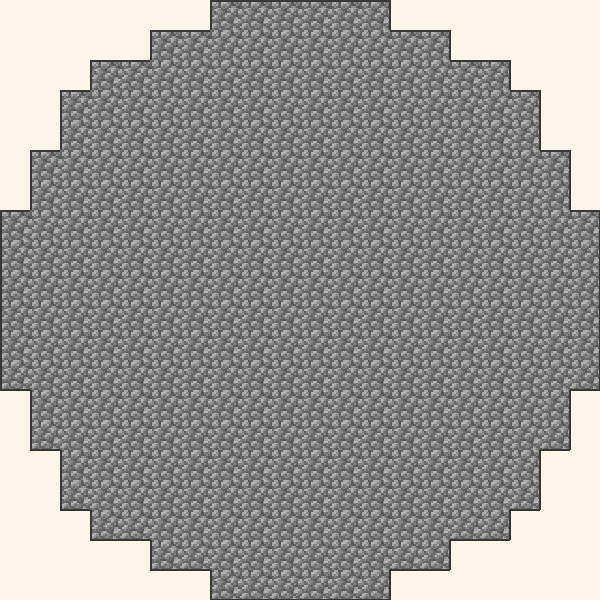
\includegraphics[width=\linewidth]{fig04_2d_d20_euclidean.png}
  \caption{\emph{塗りつぶし}}
\end{subfigure}\hfill
\begin{subfigure}[t]{0.31\linewidth}\centering
  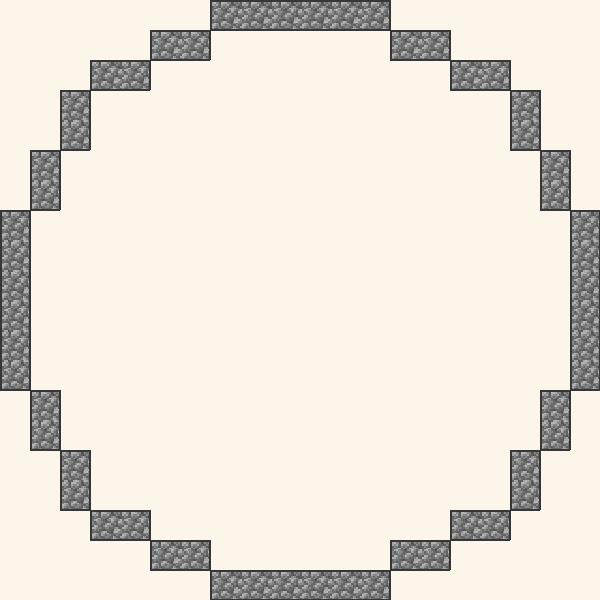
\includegraphics[width=\linewidth]{fig08_2d_d20_thin.png}
  \caption{\emph{薄壁}（1ブロック外殻）}
\end{subfigure}\hfill
\begin{subfigure}[t]{0.31\linewidth}\centering
  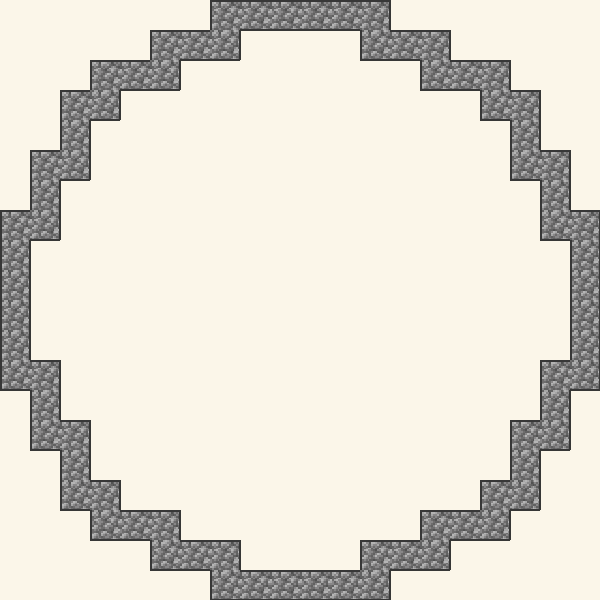
\includegraphics[width=\linewidth]{fig09_2d_d20_thick.png}
  \caption{\emph{厚壁}（対角を埋めた外殻）}
\end{subfigure}
\caption{同じユークリッド円（直径20）に対する三つの描画モード。\emph{薄壁}モードは離散的なトポロジカル境界に対応。\emph{厚壁}モードは45°方向の穴を防ぐためにブロックを追加する。これはマインクラフトの水中 Glass ドームで生じる現象そのものだ。対角の隙間から水が浸入してしまうのを防ぐ。}
\label{fig:render-modes}
\end{figure}

\subsection{ブロックのテクスチャ：Block Round の独自性}

どのボクセルを置くかという\emph{数学はテクスチャから独立している}が、Block Round は各ボクセルを\emph{マインクラフトの正準的な六面テクスチャ}で描画する。同じ直径10の球は、選んだブロック次第で視覚的性格を完全に変える（Figure~\ref{fig:textures}）。\emph{アルゴリズムは一切変わっていない}。これが本指導案の中核的な学習ポイントである。\emph{形は数学から、見た目は事後の美的決定から生まれる}。

\begin{figure}[!htbp]
\centering
\begin{subfigure}[t]{0.31\linewidth}\centering
  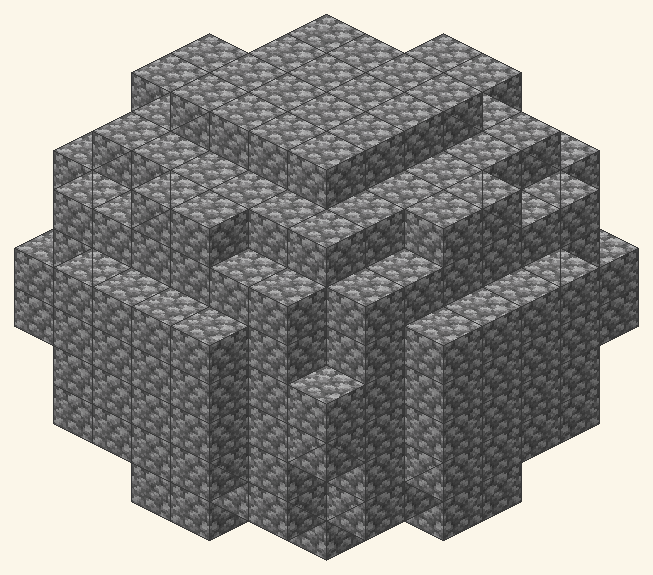
\includegraphics[width=\linewidth]{fig15_3d_sphere_cobblestone.png}
  \caption{\emph{Cobblestone}}
\end{subfigure}\hfill
\begin{subfigure}[t]{0.31\linewidth}\centering
  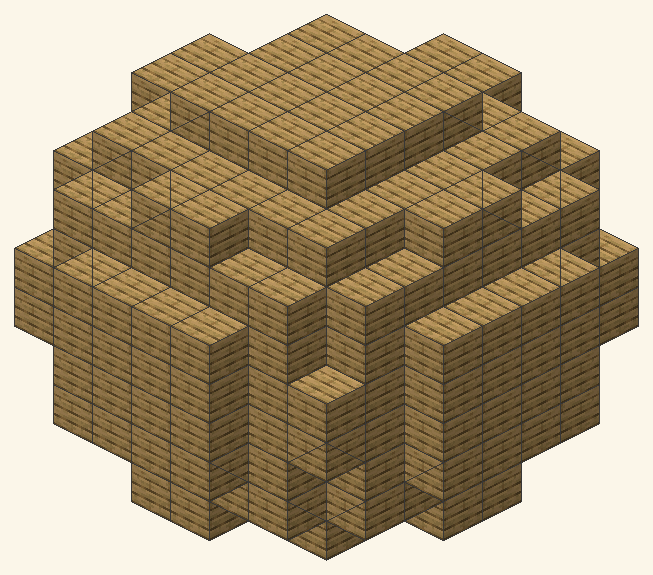
\includegraphics[width=\linewidth]{fig17_3d_sphere_oak.png}
  \caption{\emph{Oak Planks}}
\end{subfigure}\hfill
\begin{subfigure}[t]{0.31\linewidth}\centering
  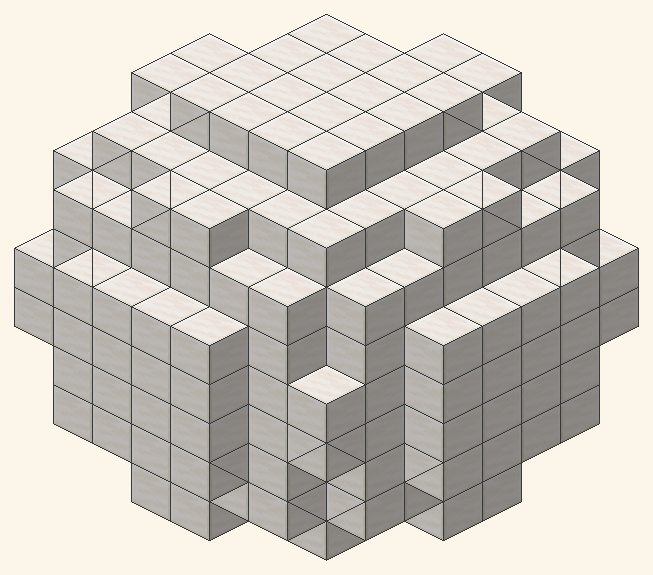
\includegraphics[width=\linewidth]{fig19_3d_sphere_quartz.png}
  \caption{\emph{Quartz Block}}
\end{subfigure}
\caption{同じ直径10の球に三種類のマインクラフトのテクスチャを適用したもの。ボクセル化された輪郭は三つとも同一---数学は変わっていない。変わるのは視覚的性格だ。\emph{Cobblestone}は中世の城壁を想起させ、\emph{Oak Planks}は山小屋か船の内装を、\emph{Quartz Block}は現代的な神殿（白を基調とする日本の伝統美にも通じる）を想起させる。}
\label{fig:textures}
\end{figure}

% =============================================================================
\section{既習事項}\label{sec:prerrequisitos}

本指導案は次の事項に既に触れていることを想定する。

\begin{itemize}[leftmargin=1.3em,itemsep=0.15em,topsep=0.3em]
  \item 平面座標：点 $(x, y)$ と $(x, y, z)$ の位置決定（数学I・II）。
  \item 円の方程式（数学II「図形と方程式」）。
  \item 多角形と円の面積、立方体・角柱・円柱の体積（数学I・A）。
  \item 関数の概念：定義域、値域、グラフ。
  \item 比と百分率。
  \item 整数の割り算における商と余り（数学A・中学校既習）。
\end{itemize}

\emph{任意の予備知識（必須ではないが有用）：}マインクラフトへの親しみ。本指導案は、マインクラフトを\emph{まったく}遊んだことのない生徒（離島や山間部の高校では起こりうる）でも完全についていけるよう設計されている。すべての操作は Block Round 上で完結する（自己完結したブラウザ内のアプリ）。

万が一、上記の必須事項に弱点がある場合（コロナ禍以降の数学的基礎力低下は OECD PISA 数学リテラシーや国立教育政策研究所「全国学力・学習状況調査」高校段階追跡で確認されている）、第1授業に\emph{診断的・補修的}な10分の時間を確保している。§\ref{aula1} を参照。

% =============================================================================
\section{教材・教具}\label{sec:recursos}

\subsection{デジタル教材}
\begin{itemize}[leftmargin=1.3em,itemsep=0.15em,topsep=0.3em]
  \item Block Round（生徒1人につき1台、または1組につき1台）。
  \item プロジェクタ、HDMI入力付きTV、または電子黒板。
  \item \emph{情報科教室}の共用端末、または\emph{BYOD}（Bring Your Own Device、生徒所有スマートフォン・タブレット）、または GIGAスクール構想で配備された端末。
  \item（任意、第5授業）マインクラフト Java版またはマインクラフト教育版（mod \emph{Litematica} または \emph{Schematica} 導入推奨）、もしくはバニラの \cmd{/fill}・\cmd{/clone} を使用。
\end{itemize}

\subsection{アナログ教材}
\begin{itemize}[leftmargin=1.3em,itemsep=0.15em,topsep=0.3em]
  \item 5mm 方眼紙、生徒1人につき2枚。
  \item HBの鉛筆、消しゴム、30cm 定規。
  \item 色鉛筆またはサインペン（特に Block Round のパレットの草色 \texttt{\#5B8E3F} と土茶色 \texttt{\#825432}）。
  \item 演習問題プリント（付録~\ref{ap:exerc}）。
  \item 黒板またはホワイトボード。
\end{itemize}

\subsection{教科書と検定教科書制度}\label{sec:pnld}

Block Round は、文部科学省検定を経た教科書を\emph{補完}するものであって代替するものではない。本指導案の内容と直接連動する教科書出版社・シリーズ（数学II・C を中心に）：

\begin{itemize}[leftmargin=1.3em,itemsep=0.1em,topsep=0.2em,nosep]
  \item 数研出版『チャート式 数学II』『チャート式 数学C』（青チャート・黄チャート・白チャート）。
  \item 東京書籍『新編数学II』『新編数学C』。
  \item 啓林館『改訂版 数学II』『改訂版 数学C』。
  \item 数研出版『改訂版 教科書 数学II』『改訂版 教科書 数学C』。
  \item 実教出版『新版 数学II』『新版 数学C』。
\end{itemize}

これらの\emph{円の方程式}、\emph{二次曲線}、\emph{平面・空間ベクトル}、\emph{微分積分の応用としての体積}を扱う章が、本指導案と直接対話する。特に\emph{タイリング}・\emph{被覆}・\emph{格子上の計数}に関する発展問題（チャート式の章末問題に頻出）は、Block Round の中心問題とほぼ等価で、用語が異なるだけである。

\subsection{Block Round へのアクセス}

優先順位に従って：

\begin{enumerate}[leftmargin=1.5em,itemsep=0.15em,topsep=0.3em]
  \item \textbf{教員による配信}：GitHub Pages 公開版を黒板に映した QR コードで配信。公開URL：\url{https://vinisouza128.github.io/block-round/}。
  \item \textbf{ローカルコピー}：情報科教室のフォルダにファイルをコピーして、\emph{file://} プロトコルで実行。
  \item \textbf{スマートフォンへのオフライン}（PWA）：一度ネット接続で開けば、ブラウザがアプリとしてインストールできる。以降はオフライン動作可能。
\end{enumerate}

% =============================================================================
\section{日本の多様な学校現場への適応}\label{sec:adapt}

日本の高校は多様である。学習指導要領は全国共通だが、生徒層・地域・課程・進路は学校ごとに大きく異なる。本指導案はその多様性に対応するよう設計されている。

\subsection{都市部の公立進学高校・中高一貫校}
東京（都立日比谷・西・国立など）、横浜（神奈川県立横浜翠嵐・湘南など）、大阪（北野・天王寺・大手前など）、京都（堀川探究科）、福岡（修猷館・福岡など）、私立中高一貫校（麻布・武蔵・桜蔭・女子学院・開成・灘・東大寺学園など）。情報科教室・電子黒板・Wi-Fi が整備されていることが多い。マインクラフト教育版のライセンスを契約済みの学校もあり、第5授業をそのままマインクラフト教育版で実施できる。\emph{本指導案を情報科教室で完全実施するのに最も適した環境}。SSH 指定校では課題研究の素材としても活用可能。

\subsection{地方の県立公立高校（県庁所在地〜中規模都市）}
全国の県立高校の多数を占める。情報科教室は機能しているが、整備に差がある。\emph{BYOD モデル}を推奨：生徒のスマートフォンを2人組で1台、Block Round を起動。2018年以降の Android/iOS なら快適に動作する。マインクラフトを校内で利用できない場合、第5授業はコマンドを紙の上で計画する形式に切り替え可能（概念学習は損なわれない）。\acc{日本の高校の典型}的環境。

\subsection{工業科・商業科・農業科・水産科などの専門学科と高等専門学校（高専）}
高専は5年制の国立教育機関（53校 + 公立3校 + 私立3校）で、本指導案の高校3年は本科3年次に相当する。技術系の素養が高く、Block Round の数学を Python・C・JavaScript で再実装することが可能。第2授業（ブレゼンハム）は情報科目との連動で深掘り、第5授業はマインクラフト Java サーバを構内に立てて協働建築の対象にできる（高専のロボコン・プロコン・デザコンの活動と接続）。工業科の\emph{機械製図}・\emph{CAD}、商業科の\emph{ビジネス情報}、農業科の\emph{農業情報処理}、水産科の\emph{海洋情報処理}との教科横断が容易。

\subsection{離島・過疎地の高校（北海道・東北・九州・沖縄）}
北海道の道東・道北、東北の三陸・日本海側、九州の宮崎・鹿児島、沖縄県の離島（宮古・八重山・大東諸島）など。情報インフラは均一でない。\emph{Block Round のオフライン PWA 動作}が決定的に有用。教員所有の1台と方眼紙を組み合わせる構成、または付録~\ref{ap:adapt-analog} の完全アナログ実施で対応できる。第3授業は、地域の伝統建築（沖縄の赤瓦屋根・石垣・グスク・古墳、北海道のチセ、東北の合掌造り・茅葺き）の幾何学的観察と接続させると教育効果が高い。

\subsection{アイヌ民族や在日コリアン・新興留学生・帰国生徒が多い学校}
札幌・苫小牧・帯広・釧路の一部高校（北海道沿岸）、沖縄県・離島の高校、大阪生野区の一部高校、神戸の一部高校、浜松・豊橋・群馬太田のブラジル人学校に接続する公立高校など。\emph{多文化共生}の視点で、第3授業の\emph{日本伝統幾何文様}（麻の葉・青海波・七宝・籠目・市松・矢絣）と並べて、\emph{各民族の幾何学伝統}（アイヌのチセ建築のシンメトリー、ウチナーグチの石垣・グスクの曲線、朝鮮半島の伝統文様）を扱える。\emph{アイヌ民族支援法}（令和元年2019年）と\emph{外国人児童生徒等教育の充実方策について}（文部科学省・平成28年）の趣旨に沿う実践となる。

\subsection{スーパーサイエンスハイスクール（SSH）指定校}
文部科学省が指定する約220校（令和5年度時点）。理科・数学・情報の研究を重視する。本指導案を\emph{課題研究}のテーマとして発展させられる。例：「三つのアルゴリズムの誤差を $D \to \infty$ で解析的に評価する」「ボクセル化の対称群を分類する」「日本伝統文様の幾何学的階級分けと自動生成」「3Dプリンタによる物理化と精度評価」。SSH 成果発表会・サイエンスアゴラ・科学の甲子園・数学甲子園での発表素材となる。

\subsection{定時制・通信制・高等専修学校（社会人・成人学習者）}
午後・夜間の定時制、通信制、高等専修学校（高等課程）、単位制高校、NHK学園、放送大学への移行を視野に。1コマあたりの時間が短いことが多いので、各活動を20\%短縮し、長文の記述を省き口頭討議を優先する。第5授業（マインクラフト実建築）は\emph{任意}とし、第1〜第4授業の概念学習を中心に据える。社会人学習者の多くはマインクラフトに馴染みがある（子どもと一緒に遊んだ世代、初期からのプレイヤー）ため、導入の障壁は低い。

\subsection{100分連続授業（2時限連続）への変換}
\emph{二単位時間連続}のスケジュール（高専・SSH の一部、課題研究の時間、土曜講座）に対応するため、第1+第2授業を1単元（100分）、第3+第4授業を1単元（100分）、第5授業を単独単元（50分または100分）として再編できる。総時数：100分×2回 + 50分×1回（合計250分）、または 100分×2.5回。

\subsection{都道府県教育委員会・地域カリキュラムとの対応表}

主要な都道府県教育委員会で、本指導案と関連する単元・特色プログラムは次の通りである。

\begin{center}
\small
\begin{tabularx}{\textwidth}{@{}p{0.18\textwidth}p{0.25\textwidth}X@{}}
\toprule
\textbf{教育委員会} & \textbf{該当する単元} & \textbf{特色プログラム} \\
\midrule
東京都教育委員会 & 数学II・C「図形と方程式」「平面上の曲線」 & 進学校多数、SSH指定多、Tokyo Global Gateway 連携可能。 \\
\addlinespace[3pt]
大阪府教育委員会 & 数学II・III・C 球と楕円体の体積 & 公立高校改革、文理学科・グローバル科の課題研究。 \\
\addlinespace[3pt]
神奈川県教育委員会 & 数学II・C 図形と座標 & 横浜・川崎の大都市圏、SSH多数、ICT先進校。 \\
\addlinespace[3pt]
京都府教育委員会 & 数学II・C 二次曲線 & 堀川高校探究科、洛北高校サイエンス科。 \\
\addlinespace[3pt]
沖縄県教育委員会 & 数学II 図形と方程式 & 離島・観光科・国際情報科の課題研究、地域文化との接続。 \\
\addlinespace[3pt]
北海道教育委員会 & 数学II・C 図形と方程式・二次曲線 & 広域・冬季の遠隔教育、農業高校・水産高校との連携。 \\
\addlinespace[3pt]
福島県教育委員会 & 数学II・C 図形と方程式 & 東日本大震災後の再生プロジェクト、SSH多数（福島・郡山・会津）。 \\
\bottomrule
\end{tabularx}
\end{center}

\subsection{ハイブリッド・遠隔授業}
Block Round の Web ベースという性質により、遠隔授業（Google Classroom for Education、Microsoft Teams for Education、Manabi Pocket、ロイロノート・スクール、Classi、すらら等のクラウド学習プラットフォーム）に自然に統合できる。教員が画面を共有し、生徒は自端末で並行操作する。方眼紙の活動は、スマートフォンで撮影し、課題提出用クラウド（Classi、Studyplus 等）に\emph{非同期}でアップロードできる。第5授業は共有マインクラフトサーバー（Realms、または学校サーバー）で実施し、生徒は仮想世界で集合して協働建築できる。

% =============================================================================
\section{授業計画}\label{sec:sequencia}

本シーケンスは、\acc{動機づけ → 課題提起 → 体系化 → 統合}という構造を採る。これはブラジルの Delizoicov \& Angotti（1990）の「三つの教育的瞬間」に着想を得ているが、日本の数学教育における伝統的な「導入・展開・まとめ」とも整合する。各50分授業は、若い高校生の認知リズムに配慮し、15分以下の説明的展開と実践的活動を交互に配置する。

% =============================================================================
\subsection{第1授業 ---「ゲームはどうやって立方体だけで球を描くのか？」}\label{aula1}

\subsubsection*{授業の目標}
離散ラスタライゼーションを\emph{真正の数学問題}として位置づけ、円の方程式を動員し、Block Round を導入する。本日の中心的問題、すなわち\emph{「どのブロックを置くか、どのように決めるのか？」}が、マインクラフトで球を建てる時にすべてのプレイヤーが直面している問題そのものであることを認識させる。

\begin{katsudou}[1.1 --- 動機づけ \quad\tempo{10分}]
\textbf{方略：}\emph{Think--Pair--Share}（個人で考え、ペアで対話し、クラスで共有する）。 \\[0.4em]
\textbf{手順：}
\begin{enumerate}[leftmargin=1.5em,itemsep=0.2em,topsep=0.3em,nosep]
  \item マインクラフトの定番建築を3例投影（または黒板に描く）。Stone の土台に Glass のドームを乗せた構造（日本語チュートリアルなら多数）。日本のマインクラフトサーバー（例：マインクラフトカップ全国大会の優勝作品、学校サーバーの作例）で建てられた\emph{巨大球体}。日本のキャラクター（ピカチュウ、ドラえもん、サンリオキャラ、東京タワー、富士山）の ピクセルアート。
  \item 生徒に問う：「\emph{よく見てください。ゲームは立方体しか置けないのに、どうやって球の形を作っているのでしょうか？マインクラフトは魔法のコンパスを内蔵しているのですか？}」
  \item 生徒は1分で個人ノートに記録し、続いて2分で隣席のペアと討議する。
  \item 全体共有：黒板の隅にキーワードを書き留める。「ゲームは立方体しか置けない。\emph{ではどの立方体を置くかを誰がどう決めているのか？}」という核心の観察に導く。
\end{enumerate}
\end{katsudou}

\begin{katsudou}[1.2 --- 課題提起 \quad\tempo{15分}]
\textbf{方略：}手描き作図と形式的定義との照合。 \\[0.4em]
\textbf{教具：}方眼紙、鉛筆。 \\[0.4em]
\textbf{手順：}
\begin{enumerate}[leftmargin=1.5em,itemsep=0.2em,topsep=0.3em,nosep]
  \item 生徒は方眼紙の半分を受け取り、$11 \times 11$ セル領域の中心を1点定める。
  \item 指示：「\emph{直径10（半径5）の最善の円を描いてください。\emph{1マスはマインクラフトの cobblestone 1ブロックだと考えてください}。時間は4分。}」
  \item 終了後、3〜4名が黒板に出て、黒板上の格子（チョーク・マーカで描いたもの）に自分の図を再現する。
  \item 教員主導の観察：「\emph{見てください。皆さん同じ図を描いたでしょうか？違いますね。なぜでしょう？どれが正解でしょうか？クラスで共有するマインクラフトサーバーで、皆さんがバラバラのドームを建ててしまったら、どんな問題が起こるでしょうか？}」
  \item まとめ：唯一の答えはない（§\ref{sec:justificativa} で示した Figure~\ref{fig:comp-d10} がそれを示している）。各生徒は暗黙のうちに異なる\acc{判定基準}を採用していた。
\end{enumerate}

\textbf{民族数学的補足：}\emph{この回答の多様性こそが民族数学の研究対象である}、と教員はここで触れる。ブラジルのウビラタン・ダンブロジオが体系化したこの研究領域は、異なる文化・集団が同じ問題を異なる方法で同等に正しく解くことに注目する。日本では遠山啓・銀林浩・横地清・横山悦郎らが類似の問題意識を展開してきた。\emph{日本のマインクラフト共同体自体が独自の「民族数学」を持つ}と言える。YouTube の日本語チュートリアル、日本人作のmod、日本国内マインクラフトサーバーで継承される建築知の体系である。
\end{katsudou}

\begin{katsudou}[1.3 --- 体系化 \quad\tempo{15分}]
\textbf{方略：}対話的講義（黒板を用いた解説）。 \\[0.4em]
\textbf{内容：}

原点を中心とする半径 $r$ の円の陰関数方程式は

\begin{shiki}
\centering
$\displaystyle x^2 + y^2 \;=\; r^2$
\end{shiki}

円の\emph{内部}の点は $x^2 + y^2 < r^2$、\emph{外部}の点は $x^2 + y^2 > r^2$ を満たす。この方程式は半軸 $r_x$、$r_y$ の楕円に一般化される：

\begin{shiki}
\centering
$\displaystyle \left(\dfrac{x}{r_x}\right)^{\!2} + \left(\dfrac{y}{r_y}\right)^{\!2} \;=\; 1$
\end{shiki}

ボクセル（ブロック）の格子上で、\acc{どのセル}が内部に属するかを決めるのが本問題である。決め方が違えば描かれる図も違う。Block Round は\emph{三つ}の基準を実装している：

\begin{itemize}[leftmargin=1.3em,itemsep=0.15em,topsep=0.3em]
  \item \acc{ユークリッド}：セルの中心 $(i + \tfrac{1}{2},\, j + \tfrac{1}{2})$ が内部にあるか？
  \item \acc{ブレゼンハム}：1965年（IBM の Bresenham 発表）の歴史的アルゴリズム。整数演算のみを用いる。
  \item \acc{閾値}：セルの\emph{隅}のいずれかが内部にあるか？
\end{itemize}

\textbf{実演：}教員が Block Round を開き、直径を10に設定、三つのアルゴリズムをクラスの観察のもとで切り替える。強調すべき点：三つの図はそれぞれ\emph{数学的に正しい}（基準が違うだけ）。さらに、アプリではブロックのテクスチャを変えられる（cobblestone、oak\_planks、diamond、glowstone）が、\emph{形は変わらない}。\emph{これが Block Round の核心：形は数学、テクスチャは美的選択}。
\end{katsudou}

\begin{katsudou}[1.4 --- 統合 \quad\tempo{10分}]
\textbf{方略：}個人による即時応用。 \\[0.4em]
\textbf{指示：}「\emph{方眼紙に戻り、直径10の円を\acc{厳密に}ユークリッド基準で描き直してください。すなわち、セルの中心 $(i + 0{,}5,\, j + 0{,}5)$ から中心までの距離が 5 以下であるとき、そのとき限り、セルを塗る。}」

完了後、紙の図と Block Round のユークリッド・直径10（Figure~\ref{fig:comp-d10}(a)）の出力を比較。\emph{一致するはず}。
\end{katsudou}

\begin{minecraft}[ゲームとの接続]
\emph{マインクラフト Java版}に WorldEdit mod を導入すると、コマンド \cmd{//sphere stone 5} は、Block Round のブレゼンハム・直径10の出力と\emph{同じ図}を描く。サーバーで遊んでいる生徒は自宅で確認できる。\emph{つまり、この授業で扱っているのは「マインクラフトの教育的シミュレーション」ではなく、マインクラフトが裏で実際に使っているのと同じ数学なのである}。
\end{minecraft}

\subsubsection*{宿題（任意）}
1.4 の作図を直径8と直径14でも実施。次回持参。マインクラフトを自宅で遊んでいる生徒は、ゲーム内で再現を試みる（\cmd{/setblock} で1個ずつ、WorldEdit があれば \cmd{//sphere} で）。撮影して提出してもよい。

% =============================================================================
\subsection{第2授業 ---「三つのアルゴリズム、三つの図、三つの建築計画」}\label{aula2}

\subsubsection*{授業の目標}
三つのアルゴリズムを「数学的に異なる定義」として深く理解し、定量的に比較する。サバイバル建築者にとっての\emph{ブロック収集量}という実践的含意も含めて検討する。

\begin{katsudou}[2.1 --- 振り返り \quad\tempo{5分}]
宿題の作図を簡単に回収し、クラス全体の傾向を観察、本日の目標を宣言：「\emph{今日は、三つのアルゴリズムを拡大鏡で観察し、なぜブレゼンハムが計算機科学の宝石とされるのか、そしてなぜ日本のマインクラフト共同体が、その名を知らずに毎日それを使っているのかを発見します。}」
\end{katsudou}

\begin{katsudou}[2.2 --- ユークリッド・アルゴリズム \quad\tempo{10分}]
形式化。セル $(i, j)$ について、正規化座標を計算する：

\begin{shiki}
\centering
$\displaystyle d_x = \dfrac{i + \tfrac{1}{2} - c_x}{r_x},\qquad d_y = \dfrac{j + \tfrac{1}{2} - c_y}{r_y}$
\end{shiki}

セルは、$d_x^{\,2} + d_y^{\,2} \leq 1$ を満たすとき、そのとき限り塗られる。

\textbf{黒板：}$c_x = c_y = 5$、$r_x = r_y = 5$、セル $(2, 1)$ の場合を明示的に解く。$d_x = (2{,}5 - 5)/5 = -0{,}5$、$d_y = (1{,}5 - 5)/5 = -0{,}7$ ゆえに $d_x^2 + d_y^2 = 0{,}25 + 0{,}49 = 0{,}74 \leq 1$。セルは\emph{内部}。 \\

生徒にセル $(0, 0)$ を試させる（結果は？）。討議。
\end{katsudou}

\begin{katsudou}[2.3 --- ブレゼンハム・アルゴリズム \quad\tempo{15分}]\label{at:23}
\textbf{歴史的文脈：}Jack Bresenham は1965年、IBM 在職時にこのアルゴリズムを発表した（\emph{IBM Systems Journal}、4巻1号、25--30ページ）。それ以前、直線を描くのに浮動小数点演算が必要で、当時のコンピュータでは高価だった。Bresenham は\emph{整数演算のみ}（加算と比較のみ）で描けることを示した。同時期、日本では\acc{FUJIC}（1956年、富士写真フイルム研究室で岡崎文次が開発）が日本初のコンピュータとして稼働しており、その後の NEC PC-9801（1982〜）、TRON プロジェクト（坂村健、1984〜）、富士通の\emph{京}（2011）、\emph{富岳}（2020、世界一位のスパコンに4部門で輝く）へと、日本の計算機の伝統は続く。

円のためのブレゼンハムは\emph{判定パラメータ} $d$ を用いる。$(x{=}0,\, y{=}R)$ から $d_0 = 1 - R$ で開始。$0$--$45^\circ$ オクタントの各ステップで：

\begin{shiki}
\centering
$\begin{cases}
\text{もし } d < 0\text{:} & \text{次：} (x{+}1,\, y),\; d \mathrel{+}= 2x+3 \\
\text{もし } d \geq 0\text{:} & \text{次：} (x{+}1,\, y{-}1),\; d \mathrel{+}= 2(x-y)+5
\end{cases}$
\end{shiki}

\textbf{黒板での実演：}$R = 5$ について段階的に追跡。$x, y, d$ を各反復で記録。残り7オクタントは対称性で得る。 \\

\textbf{マインクラフトとの接続：}WorldEdit の \cmd{//sphere} コマンド（Sponge、Bukkit、Paper、Fabric のいずれの実装でも）はブレゼンハム3Dの変種を採用している。\emph{1965年と同じ数学が、世界中の数百万のマインクラフトサーバーで現在も動いている}。誰かが \texttt{//sphere stone 8} と打つたびに、皆さんが今学んでいるのと同じ計算が裏で実行されている。

\textbf{日本情報オリンピック (JOI) との接続：}ブレゼンハムは\href{https://www.ioi-jp.org/}{日本情報オリンピック (JOI)} の予選・本選で出題される古典的トピックである。情報処理学会の関連大会、パソコン甲子園（会津大学主催）、U-22プログラミング・コンテスト等で発展問題を解いてきた高校生・高専生は多い。興味のある生徒は JOI 公式サイトの過去問・解説に進める。

\textbf{方法論的注意：}クラスが判定関数 $d$ の代数に困難を示す場合、アルゴリズムを\emph{規則}としてだけ提示すればよい（判定関数の導出は省く）。完全な正当化は技術解説書 \texttt{Block\_Round\_Math\_ja-JP.pdf} の§5にある。
\end{katsudou}

\begin{katsudou}[2.4 --- 閾値アルゴリズム \quad\tempo{10分}]
セル $(i, j)$ ごとに、中心に\emph{最も近い隅}を計算：

\begin{shiki}
\centering
$\displaystyle n_x = \mathrm{clamp}(c_x,\, i,\, i{+}1),\qquad n_y = \mathrm{clamp}(c_y,\, j,\, j{+}1)$
\end{shiki}

セルは $\left(\dfrac{n_x - c_x}{r_x}\right)^{\!2} + \left(\dfrac{n_y - c_y}{r_y}\right)^{\!2} \leq 0{,}94$ のとき塗られる。

\textbf{なぜ 1 ではなく $0{,}94$ なのか？}経験的に、1 だと東西南北の頂点に1ブロックの「棘」が現れる。閾値をわずかに下げるとそれが消える。\emph{これは目視点検による工学的決定}---理論数学が単独では足りない好例である。\emph{遠山啓}の数学教育協議会が強調した「数学と現実の対話」、すなわち最終決定権を式が独占するのではなく、理論と実践の対話で決めるという立場と通じる。

\textbf{マインクラフトで閾値が役立つ場面：}\emph{遠景から見える}ドーム（山頂の神殿、湖の島の霊廟）には、閾値アルゴリズムが少しだけ「満ちた」シルエットを生み、霧やアンビエントオクルージョン越しに視認しやすい。コスト：5--10\% のブロック増。\emph{遠景の美観}を優先するプロジェクトでは推奨。
\end{katsudou}

\begin{katsudou}[2.5 --- 定量比較 \quad\tempo{10分}]\label{at:25}
\textbf{2人組の実践活動。}Block Round（または中央プロジェクタ）で：
\begin{enumerate}[leftmargin=1.5em,itemsep=0.15em,topsep=0.3em,nosep]
  \item 直径20、\emph{塗りつぶし}モードに設定（Figure~\ref{fig:comp-d20} が結果。各アルゴリズムでの予想図）。
  \item キャンバス端の\emph{Info chip}を表示。三つのアルゴリズムそれぞれの面積を記録。
  \item 連続面積を計算：$\pi r^2 = \pi \cdot 10^2 \approx 314{,}16$。
  \item 各アルゴリズムの相対誤差を計算：$\dfrac{|\text{離散面積} - \text{連続面積}|}{\text{連続面積}} \times 100\%$。
  \item 三つを連続値から近い順に並べる。
  \item \emph{マインクラフトとの接続：}「\emph{この三つの球をサバイバルで建てるとして、どれが cobblestone の倉庫から最も少ない往復で済むでしょうか？最も多いのは？}」最小（ユークリッド）と最大（閾値）の差はパック（\emph{stack}）にして1パック分にもなる。
\end{enumerate}

\textbf{期待される結果：}ユークリッドは連続値に非常に近い（誤差2\%以下）。閾値は少し過大評価。ブレゼンハムは中間。クラス全体で確認する。
\end{katsudou}

\begin{figure}[!htbp]
\centering
\begin{subfigure}[t]{0.31\linewidth}\centering
  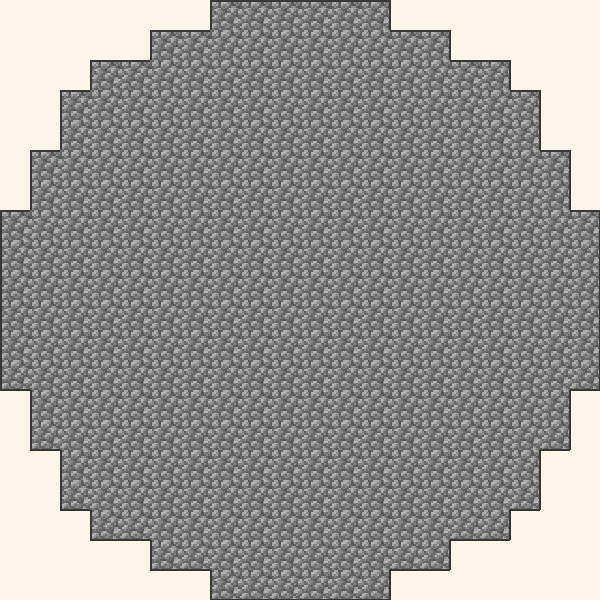
\includegraphics[width=\linewidth]{fig04_2d_d20_euclidean.png}
  \caption{\emph{ユークリッド}}
\end{subfigure}\hfill
\begin{subfigure}[t]{0.31\linewidth}\centering
  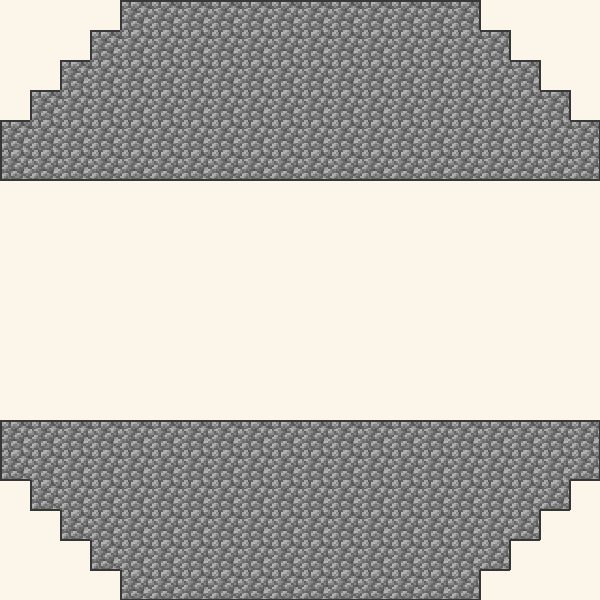
\includegraphics[width=\linewidth]{fig05_2d_d20_bresenham.png}
  \caption{\emph{ブレゼンハム}}
\end{subfigure}\hfill
\begin{subfigure}[t]{0.31\linewidth}\centering
  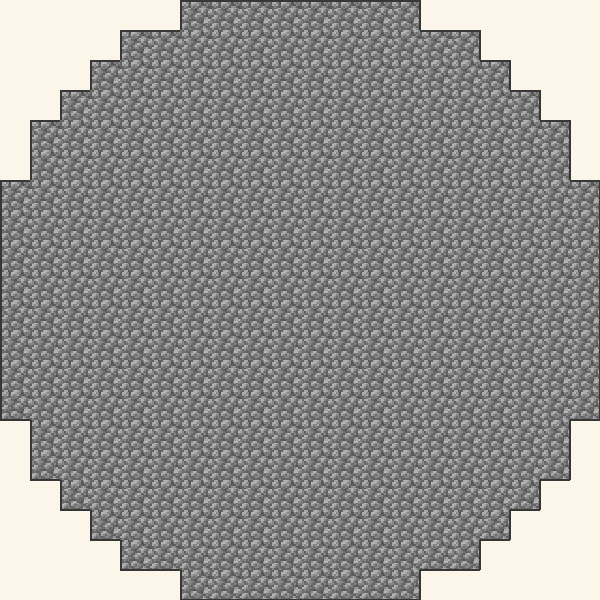
\includegraphics[width=\linewidth]{fig06_2d_d20_threshold.png}
  \caption{\emph{閾値}}
\end{subfigure}
\caption{同じ直径20の円を三つのアルゴリズムで描いたもの。cobblestone テクスチャで描画。直径が大きくなると差は微細になる---肉眼では三つとも似て見える。直径が小さいほど（Figure~\ref{fig:comp-d10}）違いがはっきりするという指摘の良い機会となる。}
\label{fig:comp-d20}
\end{figure}

\begin{minecraft}[ブロック数の比較：Block Round 対 WorldEdit]
自宅で試してみよう（マインクラフト＋WorldEdit があれば）。サーバーで \cmd{//sphere stone 10} を実行し、ブロック数を数える。Block Round の \emph{Info chip}（ブレゼンハム、$D = 20$）と比較。両者は\emph{一致するはず}（または実装上の小差異で 0--4ブロックずれる）。一貫した差異を見つけたら、それは本物の数学的発見である。
\end{minecraft}

% =============================================================================
\subsection{第3授業 ---「楕円から楕円体へ：三次元へ」}\label{aula3}

\subsubsection*{授業の目標}
楕円方程式を楕円体へ一般化し、ボクセル、離散体積計算、平面切断を導入する。日本の視覚文化伝統、および日本のマインクラフト共同体の有名作品との架橋を構築する。

\begin{katsudou}[3.1 --- 2D方程式から3Dへ \quad\tempo{15分}]\label{at:31}
平面座標 $(x, y)$ に第三座標 $z$ を加える。楕円の陰関数は自然に拡張される：

\begin{shiki}
\centering
$\displaystyle \left(\dfrac{x}{r_x}\right)^{\!2} + \left(\dfrac{y}{r_y}\right)^{\!2} + \left(\dfrac{z}{r_z}\right)^{\!2} \;=\; 1$
\end{shiki}

$r_x = r_y = r_z = r$ のとき、\acc{球} $x^2 + y^2 + z^2 = r^2$ を得る（Figure~\ref{fig:3d-shapes}）。

\textbf{ボクセル：}3D 格子のセルを\emph{ボクセル}（\emph{volume element} の短縮形）と呼ぶ。マインクラフトでは、各ボクセルが $1\times1\times1$ の\emph{ブロック}に対応する。判定基準は2Dと同形式で、$z$ 座標を加えただけ：

\begin{shiki}
\centering
$\displaystyle a_x^2 + a_y^2 + a_z^2 \leq 1,\quad \text{ただし } a_\xi = \dfrac{\xi + \tfrac{1}{2} - c_\xi}{r_\xi}$
\end{shiki}

\textbf{実演：}Block Round を3Dモードで開き、球と楕円体を切り替える。マウスで回転させ、ボクセル構造を観察。
\end{katsudou}

\begin{figure}[!htbp]
\centering
\begin{subfigure}[t]{0.45\linewidth}\centering
  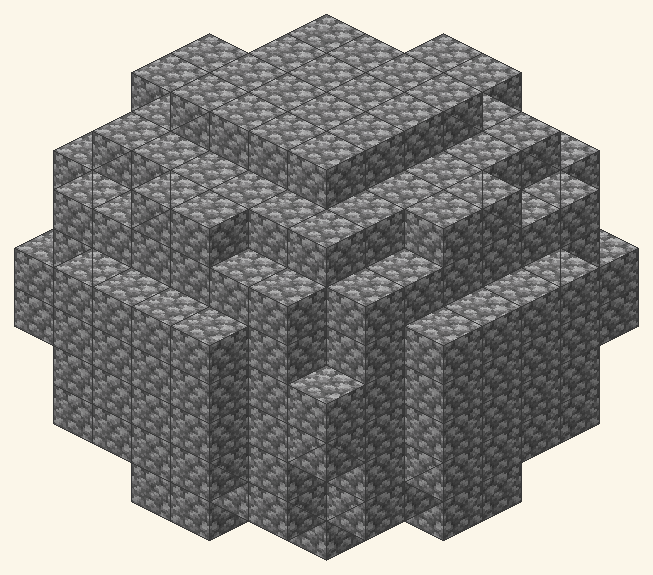
\includegraphics[width=\linewidth]{fig10_3d_sphere_d12.png}
  \caption{直径10の球（$r_x = r_y = r_z = 5$）。}
\end{subfigure}\hfill
\begin{subfigure}[t]{0.45\linewidth}\centering
  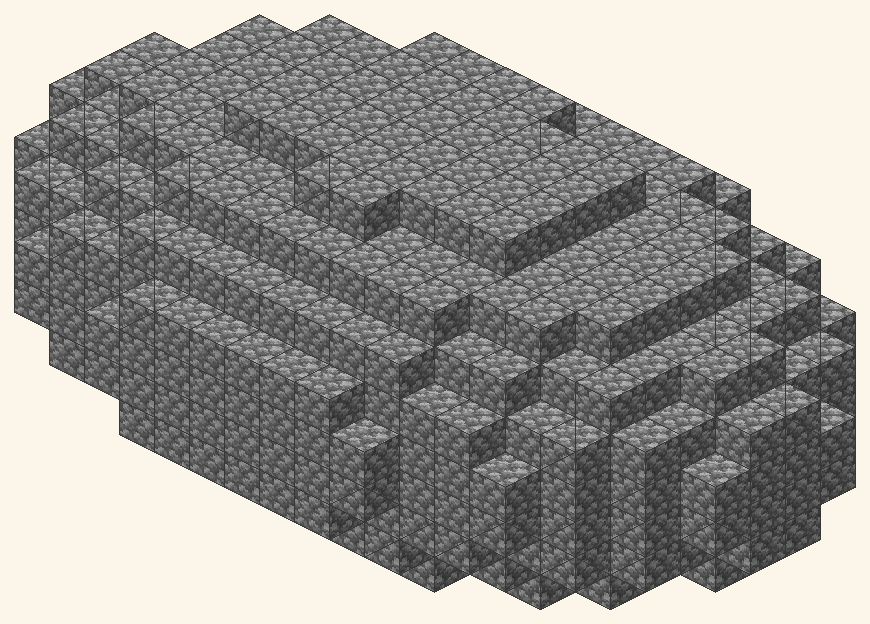
\includegraphics[width=\linewidth]{fig11_3d_ellipsoid.png}
  \caption{楕円体 $W = 20, H = 10, D = 12$。}
\end{subfigure}
\caption{3D でのボクセル化。各立方体は1ボクセル（= マインクラフトの1ブロック）であり、その中心座標 $(i, j, k)$ が陰関数方程式で判定される。表面の階段状のディテールはボクセル化の特徴---まさにマインクラフトに視覚的なアイデンティティを与えている要素である。}
\label{fig:3d-shapes}
\end{figure}

\begin{katsudou}[3.2 --- 連続体積 対 離散体積 \quad\tempo{15分}]\label{at:32}
楕円体の連続体積は古典的結果である：

\begin{shiki}
\centering
$\displaystyle V \;=\; \dfrac{4}{3}\,\pi\, r_x\, r_y\, r_z$
\end{shiki}

$r_x = r_y = r_z = r$ のとき $V = \tfrac{4}{3}\pi r^3$。これは\acc{共通テスト・個別大学2次試験で頻出}（数学C・数学III「平面上の曲線」「微分・積分」の項目で実質的に毎年問われている）であり、\hyperref[sec:jmo]{JMO} 本選の幾何問題、数学甲子園の総合問題、SSH 課題研究の素材としても活用できる。

\textbf{2人組での活動：}
\begin{enumerate}[leftmargin=1.5em,itemsep=0.15em,topsep=0.3em,nosep]
  \item 直径12の球（$r = 6$）の連続体積を計算：$V = \tfrac{4}{3}\pi \cdot 216 \approx 904{,}78$。
  \item Block Round で球 $D = 12$ を生成、\emph{塗りつぶし}モード、\emph{Info chip} を表示、離散体積（ブロック数）を記録：おおよそ $V_{\mathrm{disc}} \approx 904$ ブロック。\emph{相対誤差 $\approx 0{,}1\%$---驚異的に近い}。
  \item 同 chip 上で表記 $904 = 14 \times 64 + 8$ を観察：サバイバル建築者へのメッセージとして「\emph{cobblestone のスタックが 14個 + 部分スタック 8個 必要}」と読める。
  \item $D = 16$ で同様に実施（$V_{\mathrm{cont}} \approx 2\,144$、$V_{\mathrm{disc}} \approx 2\,145$）。$D$ が偶数の場合、誤差は\emph{正}になり得る（セル間の中心配置による過大評価）。
\end{enumerate}

\textbf{注意：}$D \to \infty$ で「離散体積 / 連続体積 $\to 1$」。$D$ が小さいときは相違が顕著---これは数学的に正しい：離散化は\emph{確かに}計数を変える。
\end{katsudou}

\begin{katsudou}[3.3 --- 平面切断 \quad\tempo{10分}]\label{at:33}
Block Round は楕円体を三つの異なる平面で切断できる。各切断はボクセル中心への\acc{一次不等式}である：

\begin{shiki}
\centering
$\begin{array}{lcl}
\text{X軸：} & x \geq \mathit{cut} & \Rightarrow \text{ボクセルを除外} \\
\text{Y軸：} & y \geq \mathit{cut} & \Rightarrow \text{ボクセルを除外} \\
\text{対角線：} & x + y \geq \mathit{cut} & \Rightarrow \text{ボクセルを除外}
\end{array}$
\end{shiki}

Figure~\ref{fig:cortes} に三つの $50\%$ 切断を示す。

\textbf{誘導討議：}「\emph{なぜ対角切断の振幅は $D_x$ ではなく $D_x + D_y$ なのか？斜辺はどこに対応するか？}」 矩形のボックス上で $x + y$ が $0$ から $D_x + D_y$ の値を取ることを認識させる。\emph{マインクラフトでは、Y方向50\%切断が球の上半分---まさに何千ものサーバーで神殿・天文台・闘技場の天蓋として用いられている古典的な「ドーム」---を生み出す。}
\end{katsudou}

\begin{figure}[!htbp]
\centering
\begin{subfigure}[t]{0.31\linewidth}\centering
  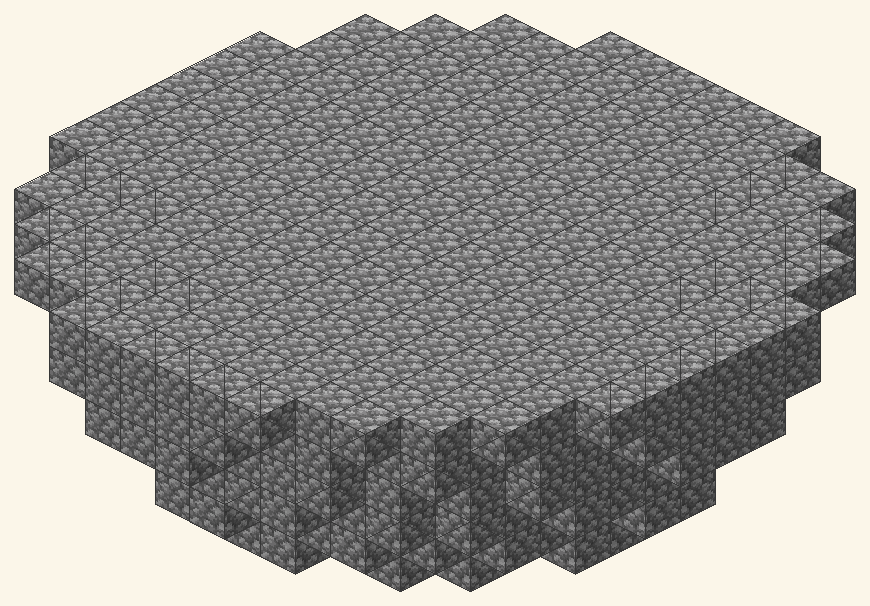
\includegraphics[width=\linewidth]{fig12_3d_cut_y50.png}
  \caption{Y軸50\% 切断 --- 古典的\emph{ドーム}。}
\end{subfigure}\hfill
\begin{subfigure}[t]{0.31\linewidth}\centering
  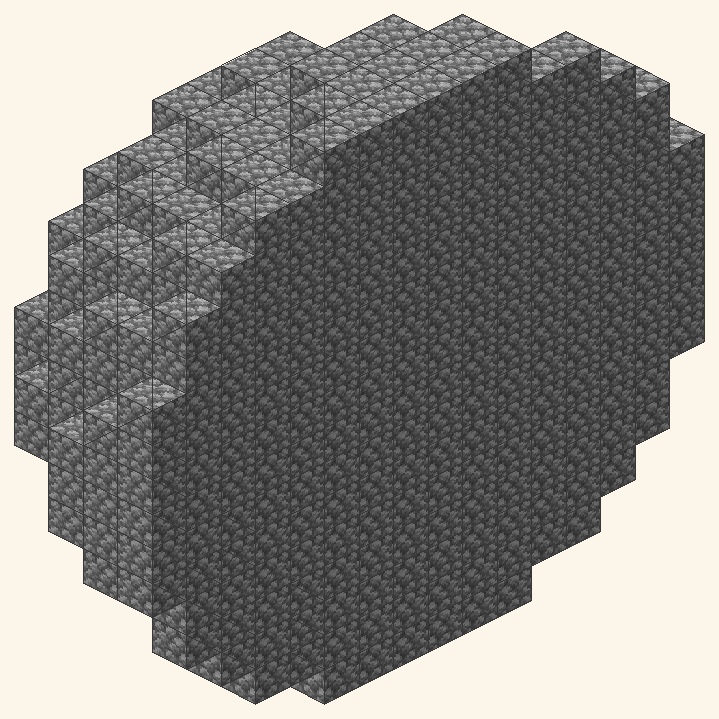
\includegraphics[width=\linewidth]{fig13_3d_cut_x50.png}
  \caption{X軸50\% 切断 --- 横の\emph{半球}。}
\end{subfigure}\hfill
\begin{subfigure}[t]{0.31\linewidth}\centering
  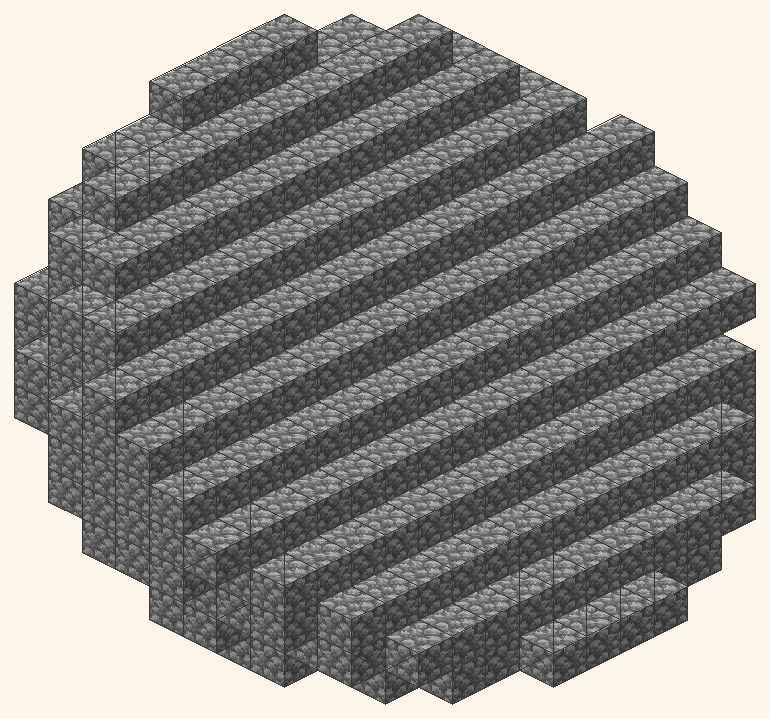
\includegraphics[width=\linewidth]{fig14_3d_cut_diag50.png}
  \caption{対角50\% 切断 --- 斜の\emph{半碗}。}
\end{subfigure}
\caption{同じ直径16の楕円体に対する三種類の平面切断、すべて50\%体積保存。対角切断の階段状パタンが目立つ---これは二軸を繋ぐ斜辺を露出させている。各切断はマインクラフトでの異なる建築計画に対応する。神殿のドーム、横向きの半競技場、噴水のある円形劇場。}
\label{fig:cortes}
\end{figure}

\begin{katsudou}[3.4 --- 日本の視覚文化遺産との対話 \quad\tempo{10分}]\label{at:34}
\emph{国語・芸術・地理歴史との接続。本活動は学習指導要領が掲げる「文化的アイデンティティと文化遺産」に関わる横断的内容を実現する。}

5つの画像を投影（または印刷配布）：

\begin{itemize}[leftmargin=1.3em,itemsep=0.2em,topsep=0.3em,nosep]
  \item \acc{国立代々木競技場}（丹下健三、1964年東京オリンピック）：吊り屋根構造、ハイパーボリック・パラボロイド曲面。鉄筋コンクリートと吊鋼索で\emph{二次曲面}を実物大で実現した世紀の建築。\emph{表参道ヒルズ}（安藤忠雄）、\emph{新国立競技場}（隈研吾、2021年東京オリンピック、木組み）、\emph{V\&Aダンディー}（隈研吾、海外作だが\emph{直接的に voxel感}を持つ）、\emph{金沢21世紀美術館}（SANAA = 妹島和世+西沢立衛、円形ガラス建築）、\emph{せんだいメディアテーク}（伊東豊雄、チューブ構造）も同様の二次曲面・離散幾何の現代的応用である。安藤忠雄の\emph{光の教会}・\emph{水の教会}・\emph{住吉の長屋}は、几何学的純化されたコンクリート建築の代表。

  \item \acc{法隆寺五重塔}（607年、世界最古の木造建築）：同心円的構造、五重の対称性。\acc{東大寺大仏殿}（世界最大級の木造建築、対称性）。\acc{六角堂・八角堂}（法隆寺夢殿、興福寺北円堂・南円堂など）：直接 $\mathbb{Z}_6$、$\mathbb{Z}_8$ 対称性。輪蔵（六角形・八角形のリビング・カルーセル）---まさに本指導案で扱う $\mathbb{Z}_2^3$ 対称性に近い。\emph{富士山}は円錐の幾何---日本人の精神的シンボル。

  \item \acc{日本伝統幾何文様}：\emph{麻の葉}（asanoha、六角に基づく星形タイリング）、\emph{青海波}（seigaiha、同心円の重なり）、\emph{七宝つなぎ}（shippō、重なり合う円のテッセレーション）、\emph{籠目}（kagome、六角の格子）、\emph{市松}（ichimatsu、チェス盤模様）、\emph{矢絣}（yagasuri、矢羽根模様）。これらすべてが\emph{日本のラスタライゼーション・ボクセルアートの先駆}である。さらに\emph{浮世絵の網点}（葛飾北斎・歌川広重・喜多川歌麿の手刷り階調表現はベン・デイ・ドット級の幾何学）、\emph{折り紙}（数理折り紙：三谷純（筑波大）、折田明子による計算折り紙）、\emph{枯山水}（karesansui、砂目の幾何学的rake）も同じ系譜にある。

  \item \acc{縄文土器}（火焔型土器、国宝、5500--4500年前）：立体的なボクセル装飾。\acc{古墳}（大仙陵古墳=仁徳天皇陵、前方後円墳、世界最大級の墳墓のひとつ）：円と四角を組み合わせた巨大\emph{voxel landscape}。\acc{埴輪}（haniwa、voxel-like ceramic figures）、\emph{銅鐸}（doutaku、弥生時代の青銅器）、\emph{弥生土器}。さらに\acc{円空仏}（江戸時代の仏師・円空の木彫り---まさにvoxel彫刻）、現代では\acc{草間彌生}の網点世界（直接的にvoxel art！）、\acc{村上隆}のスーパーフラットも同じ系譜。

  \item \acc{日本のマインクラフト共同体の代表作}：マインクラフトカップ全国大会の優勝作品、人気サーバーで建てられた都市・神殿・東京タワー再現・スカイツリー再現、日本人配信者・YouTuber（赤髪のとも、カズクラ、ヒカキン、兄者弟者、まいぜんシスターズ）の建築実況、Twitter/X 上の「\#マイクラ建築」ハッシュタグの蓄積。\emph{これが日本の現代マインクラフト民族数学の実演}である。生きていて、毎日更新され、日本語で展開されている。
\end{itemize}

\textbf{誘導討議：}「\emph{丹下健三は1964年に、皆さんが今ブロックで描いている曲面を、鉄筋コンクリートと吊鋼で実物大に建てました。隈研吾は2021年に、ボクセル感のある木組みで国立競技場を建てました。縄文時代の人々は、立体ボクセル装飾を粘土でこね、古墳時代の人々は前方後円墳という巨大な「地上ボクセル風景」を作りました。葛飾北斎は浮世絵の細かい線で階調を「ラスタライズ」しました。そして日本のマインクラフト共同体は、毎日、共有サーバーでそれを実行しています。私たちが学んでいるラスタライゼーション問題はデジタル時代の発明ではなく、人類史の通底音です。\emph{文化ごとに「ラスタライズ」の仕方が違う}のです。}」

\textbf{教科横断的接続：}芸術科・地理歴史科・地理（GIS）科の教員と連携を推奨。第4授業と第5授業では、各グループにどの\emph{日本の視覚伝統}が作品の着想源かを選択させる。
\end{katsudou}

% =============================================================================
\subsection{第4授業 ---「インベントリ算法：スタック、チェスト、コマンド」}\label{aula4}

\subsubsection*{授業の目標}
マインクラフトの\emph{インベントリ算法}を、切り上げ除算と商・余り表現の具体的応用として導入する。中心コマンド（\cmd{/fill}、\cmd{/clone}、\cmd{//sphere}、\cmd{//hsphere}）と、八面体対称性による最適化を扱う。

\begin{katsudou}[4.1 --- スタック算法 \quad\tempo{15分}]\label{at:41}
マインクラフトでは、インベントリの各スロットは最大\acc{64個の同一ブロック}を保持できる。この上限こそが体積計算に実用的意味を与える。球 $D=12$ に必要なボリュームが $V = 904$ ブロックであるとは、\enquote{ザックに904個入る}という意味ではない。\enquote{\emph{cobblestone} のスタック（満杯スロット）が $\lceil 904/64 \rceil = 15$ 個必要}という意味である。

\textbf{重要な公式：}

\begin{shiki}
\centering
$\displaystyle N_{\mathrm{stacks}} = \left\lceil \dfrac{V}{64} \right\rceil
\qquad\qquad
N_{\mathrm{large\_chest}} = \left\lceil \dfrac{V}{3\,456} \right\rceil$
\end{shiki}

（シングルチェストは27スロット、ラージチェストは54スロット。$54 \times 64 = 3\,456$ 個／ラージチェスト。）

\textbf{2人組での活動：}
\begin{enumerate}[leftmargin=1.5em,itemsep=0.15em,topsep=0.3em,nosep]
  \item 球 $D = 8$（体積 $\approx 268$ ブロック）：スタック何個？シングルチェスト何個？答え：5 スタック、シングルチェスト1個（17スロット余り）。
  \item 球 $D = 16$（体積 $\approx 2\,145$ ブロック）：スタック何個？ラージチェスト何個？答え：34 スタック、ラージチェスト1個（あと20スタックで満杯---つまり、小さなシリンダー1個分の余裕がある）。
  \item 球 $D = 32$（体積 $\approx 17\,156$ ブロック）：スタック何個？ラージチェスト何個？答え：269 スタック（$\approx$ ラージチェスト5個 + 1スタック）、$\lceil 17\,156/3\,456 \rceil = 5$ ラージチェスト。
  \item \emph{マインクラフトのサバイバルモードで、日本人プレイヤーの統計（マインクラフトサーバー\emph{JMS}や個人配信での記録）によると、cobblestone のスタック1個を入手するのに平均で4--6分かかる（つるはしの種類による）。球 $D = 16$ の総収集時間：$34 \times 5 = 170$ 分 $\approx 2{,}8$ 時間と見積もれる。}
\end{enumerate}

\textbf{数学A「整数の性質」との直接接続：}この活動はそのまま数学A「整数の性質」---「割り算の商と余り」「合同式」「ユークリッドの互除法」---の応用問題集として扱える。共通テスト数学I・A 整数問題の頻出パターンと同型である。
\end{katsudou}

\begin{katsudou}[4.2 --- マインクラフト・コマンド \quad\tempo{15分}]\label{at:42}
中心コマンドを提示：

\begin{itemize}[leftmargin=1.4em,itemsep=0.25em,topsep=0.3em]
  \item \cmd{/setblock x y z minecraft:stone} --- 特定位置に1ブロックを設置。
  \item \cmd{/fill x1 y1 z1 x2 y2 z2 minecraft:stone} --- 矩形ボックスを1種ブロックで埋める。バニラ上限：1コマンドで $32\,768$ ブロック。
  \item \cmd{/clone x1 y1 z1 x2 y2 z2 x3 y3 z3} --- 領域を別位置にコピー（対称性建築の根本的な力）。
  \item \cmd{//sphere stone 8}（WorldEdit）--- プレイヤー中心の半径8の球。ブレゼンハム3Dを使用。
  \item \cmd{//hsphere stone 8}（WorldEdit）--- \emph{中空}球（外殻のみ）。中空のドームに便利。
  \item \cmd{//ellipsoid stone 10 5 10}（WorldEdit）--- 半軸指定の楕円体 $W = 20, H = 10, D = 20$。
\end{itemize}

\textbf{実演（マインクラフトが利用可能なら）：}テスト用ワールドで \cmd{//sphere stone 8} を実行して時間を計る。Block Round の直径16・ブレゼンハム出力と比較。両者の数学的同一性を確認。

\textbf{マインクラフトが利用不可能なら：}思考実験。方眼紙に書き留める：「私は地面に立っている（y=64）。地面から8ブロック上（y=72）を中心に半径8の球を建てたい。どんなコマンド？」答え：座標 $(0, 72, 0)$ にいる状態で \cmd{//sphere stone 8}。
\end{katsudou}

\begin{katsudou}[4.3 --- 八面体対称性による最適化 \quad\tempo{15分}]\label{at:43}
\textbf{中心アイデア：}原点中心の球は三つの座標平面での鏡映に対して不変。群 $\mathbb{Z}_2^3$ は位数8。一つの\emph{オクタント}（$+x, +y, +z$ 領域）から、残り7つの領域は鏡映で得られる。

\textbf{実践的含意：}$V$ 個のブロックを一つずつ置くのではなく、オクタントに $V/8$ ブロックを建て、\cmd{/clone} で7回鏡映する。

\begin{shiki}
\centering
$\displaystyle \mathrm{Cost}_\mathrm{sym} = N_\mathrm{octant} + 7\, T_\mathrm{clone}
\;\ll\; \mathrm{Cost}_\mathrm{brute} = N\, T_\mathrm{block}$
\end{shiki}

\textbf{具体例：球 $D = 24$、中心 $(0, 72, 0)$ ：}
\begin{enumerate}[leftmargin=1.5em,itemsep=0.15em,topsep=0.3em,nosep]
  \item 手動で正のオクタントを建てる（$\approx 905$ ブロック、サバイバルで $\approx 15$ 分、クリエイティブのブラシで $\approx 45$ 秒）。
  \item $-x$ への鏡映：\cmd{/clone 0 72 0 12 84 12 -12 72 0 mode:masked}
  \item $-y$ への鏡映：\cmd{/clone 0 72 0 12 84 12 0 60 0 mode:masked}
  \item $-z$ への鏡映：\cmd{/clone 0 72 0 12 84 12 0 72 -12 mode:masked}
  \item オクタント $(-x, -y)$、$(-y, -z)$、$(-x, -z)$、$(-x, -y, -z)$：類似のコマンド。
\end{enumerate}

\textbf{時間比較：}
\begin{itemize}[leftmargin=1.3em,itemsep=0.1em,topsep=0.2em,nosep]
  \item 対称性なし、サバイバルで：$7\,238$ ブロック × 2秒/ブロック $\approx$ 4 時間。
  \item 対称性あり：15 分（オクタント）+ 0,5秒（7クローン）$\approx$ 15 分。
  \item 加速率：\emph{16倍}。
\end{itemize}

\textbf{数学C・数学B「ベクトル」との接続：}座標反射 $(x, y, z) \to (-x, y, z)$ などは、線形代数的にはベクトル空間の自己同型である。群 $\mathbb{Z}_2^3$ は\emph{離散群論}の入門題材で、JMO 本選レベルの整数問題・組合せ問題でも頻出。
\end{katsudou}

\begin{katsudou}[4.4 --- 応用：実ドームの計画立案 \quad\tempo{5分}]
2人組で、安藤忠雄風の Quartz $D=20$ ドームを縄文土器風土台または法隆寺風五重塔の屋根に据える建築計画を立てる（\emph{紙の上または Block Round で}）。記入：
\begin{itemize}[leftmargin=1.3em,itemsep=0.1em,topsep=0.2em,nosep]
  \item ドームの体積（球 $D=20$ の半分）：$\approx 2\,094$ ブロック。
  \item 必要スタック数：33 スタック。
  \item Quartz Block 数（1個につき Nether Quartz 4個必要、ネザーで採掘）：$\sim 2\,094 \times 4 = 8\,376$ Nether Quartz。
  \item 対称性を活用した最適化済みコマンド列。
\end{itemize}

この活動が第5授業（実建築）の準備となる。
\end{katsudou}

% =============================================================================
\subsection{第5授業 ---「実建築：Block Round からマインクラフトへ」}\label{aula5}

\subsubsection*{授業の目標}
これまでの内容のすべてを\emph{制作物}として動員する：Block Round から出力し、マインクラフトに（Litematica または Schematica で）読み込み、クリエイティブまたはサバイバルで実建築を行う。数学的選択の弁明的論証と最終成果物の提出によって学習を評価する。

\begin{katsudou}[5.1 --- 課題の提示 \quad\tempo{5分}]\label{at:51}
\textbf{指示：}「\emph{2人組または3人組で、Block Round で生成した三つ以上の図形（円・楕円・球・楕円体）を組み合わせたマインクラフト建築（マインクラフトが利用できなければ Block Round のみで完結する作品）を制作してください。クラスのサーバー内の都市、神殿、円形の農場、天文台---何でも構いません。最後に、各グループは作品を発表し、各選択の\acc{数学的根拠}を述べます。なぜそのアルゴリズム？なぜその比？なぜその切断？なぜそのブロック？}」
\end{katsudou}

\begin{katsudou}[5.2 --- 出力と読み込み \quad\tempo{15分}]\label{at:52}
Block Round からマインクラフトへのフローを実演：

\begin{enumerate}[leftmargin=1.5em,itemsep=0.2em,topsep=0.3em]
  \item Block Round で目的の図形を設定（例：Quartz の球 $D = 12$、Y切断50\%）。
  \item キャンバス右上の\emph{Export Schematic}ボタンをクリック。\texttt{.schem} ファイル（Sponge Schematic v2）がダウンロードされる。
  \item マインクラフト Java版に mod \emph{Litematica}（無料）を導入した状態で：mod を開き、\emph{Load Schematic}、ダウンロードしたファイルを選択。
  \item Litematica はプレイヤーが指定した位置に建築の半透明な\emph{ゴースト}を表示する。
  \item プレイヤーは\emph{ゴーストに沿って}各ブロックを置く。Litematica は位置ズレを赤で警告する。
  \item \emph{代替経路 \cmd{//schem load}：}WorldEdit のあるサーバーでは、\cmd{//schem load <filename>} でファイル名を指定して \texttt{.schem} を読み込み、\cmd{//paste -a} で現在位置に瞬時に貼り付け。
\end{enumerate}

\textbf{マインクラフトが利用不可能なら：}\texttt{.schem} のダウンロードを実演し、バイナリエディタでファイルを開いて Sponge Schematic v2、gzip、NBT の形式について討議。情報科の「データの表現」（情報I）、高専・専門学科の「情報処理」「データベース基礎」に直結する素材となる。
\end{katsudou}

\begin{katsudou}[5.3 --- 制作 \quad\tempo{20分}]\label{at:53}
\textbf{グループの教材：}
\begin{itemize}[leftmargin=1.3em,itemsep=0.15em,topsep=0.3em,nosep]
  \item Block Round へのアクセス（パソコンまたはスマートフォン）。
  \item（任意）マインクラフト + Litematica または Schematica。
  \item 下絵と計画のための方眼紙・鉛筆・色鉛筆。
  \item 義務化された3問の質問用ワークシート（付録~\ref{ap:exerc} の問題8）。
\end{itemize}

\textbf{グループ作業の内部工程：}
\begin{enumerate}[leftmargin=1.5em,itemsep=0.15em,topsep=0.3em,nosep]
  \item \tempo{5分} ブレインストーミングと紙の下絵。
  \item \tempo{8分} Block Round での制作と \texttt{.schem} 出力。
  \item \tempo{5分}（利用可能なら）マインクラフトへの読み込みと簡易テスト。
  \item \tempo{2分} ワークシートへの数学的根拠の記入。
\end{enumerate}

\textbf{教員の巡回支援：}各グループを回り、媒介的な問いかけを行う。「\emph{なぜそのアルゴリズムを選びましたか？その切断はどんな不等式で表せますか？Quartz のラージチェストは何個必要ですか？}」
\end{katsudou}

\begin{katsudou}[5.4 --- 発表と全体まとめ \quad\tempo{10分}]\label{at:54}
各グループは2分でクラスに作品を発表する。プロジェクタで投影（またはマインクラフト内で、または紙の上で）し、義務化された3問のうち\emph{少なくとも一つ}に答える。

\textbf{発表の最低基準：}
\begin{itemize}[leftmargin=1.3em,itemsep=0.1em,topsep=0.2em,nosep]
  \item 含まれる数学的図形を少なくとも一つ識別する。
  \item 選択したアルゴリズム名を述べ、その視覚効果が他のアルゴリズムでは得られないことを（\emph{事後的にでも}）正当化する。
  \item 3D 切断があれば、それを不等式で記述する。
  \item 必要なスタック・ラージチェスト数を（粗くでよいので）見積もる。
\end{itemize}

\textbf{教員による最終まとめ（3分）：}本シーケンス全体の核心---\emph{「ボクセルの離散格子の上で、同じ連続曲線は複数の表現を許す。一つを選ぶことは数学的決定であり、それをマインクラフトで建てることはシティズンシップ、資源管理、美的選択の決定でもある」}---を再確認し、現代日本数学の地平に位置づける。\hyperref[sec:jmo]{JMO/JOI}、SSH 課題研究、マインクラフトカップ全国大会への挑戦を促す。日本の3人のフィールズ賞受賞者（小平邦彦1954、廣中平祐1970、森重文1990）や、京都大学数理解析研究所 RIMS の世界的水準について短く触れて締めくくる。
\end{katsudou}

\begin{minecraft}[拡張の可能性]
この第5授業は、課外活動への複数の拡張を開く。
\begin{itemize}[leftmargin=1.3em,itemsep=0.15em,topsep=0.3em,nosep]
  \item \textbf{数学都市プロジェクト：}クラスで学校サーバーに都市を建築。各建物が一つの幾何図形（円柱、球、楕円体、二次曲線の集合）を実装。
  \item \textbf{日本文化遺産の再現：}マインクラフトで法隆寺五重塔、東大寺大仏殿、姫路城、富士山、東京タワー、スカイツリー、新国立競技場、国立代々木競技場、各地の古墳の再構築。前方後円墳（楕円体 + 円錐 + 矩形の組合せ）は本指導案の知識を総合的に動員できる素材。
  \item \textbf{Block Round オリンピック：}クラス内競技---誰が連続体積に最も近い球を建てるか？誰が対称性で最大の高速化を実現するか？
  \item \textbf{工学への接続（高専・専門学科）：}Block Round を前工学的サンドボックスとして使用：測地ドーム、ボクセル化されたトラス、滑らかな曲面を近似する離散構造。\emph{機械製図 CAD}・\emph{建築設計}との接続。
  \item \textbf{プログラミングへの接続（JOI、情報I・II）：}三つのアルゴリズムを Python または Scratch で再実装し、Block Round の出力と比較。課題研究、JOI への足がかりに。
  \item \textbf{マインクラフトカップ全国大会への参加：}文部科学省後援の公式コンテストで本指導案の成果を発表素材として活用できる。SDGs等の年度テーマと結びつけて応募。
\end{itemize}
\end{minecraft}

% =============================================================================
\section{評価}\label{sec:avaliacao}

評価は\acc{形成的・過程的・総括的}の三層で実施し、四つの次元（マインクラフト応用の独立次元を加えて五つ）を組み合わせる。日本の数学教育における「観点別評価」---知識・技能、思考・判断・表現、主体的に学習に取り組む態度---の三観点に対応するよう設計してある。

\subsection{診断的評価}
第1授業の活動1.2（円の手描き）で実施。教員は平面座標、円の方程式、計数の各点について生徒の困難を把握できる。コロナ禍以降の数学的基礎力の不均一さに対応する。

\subsection{形成的評価}
全5授業で分散実施。\emph{Think--Pair--Share} での参加と発言の質、活動~\ref{at:25}、\ref{at:32}、\ref{at:41} の計算結果を\emph{即時}フィードバック。

\subsection{総括的評価}
2つの提出物で構成される。

\begin{enumerate}[leftmargin=1.5em,itemsep=0.2em,topsep=0.3em,nosep]
  \item \textbf{演習問題集}（付録~\ref{ap:exerc}）：8問、第5授業終了時または別途指定日に提出。
  \item \textbf{最終プロジェクト}（活動~\ref{at:53}）：発表（活動~\ref{at:54}）でワークシートを口頭で答える形式。
\end{enumerate}

\subsection{評価ルーブリック}

\begin{center}
\small
\begin{tabularx}{\textwidth}{@{}p{0.21\textwidth}XX@{}}
\toprule
\textbf{観点} & \textbf{十分達成（8--10）} & \textbf{おおむね達成（5--7）／不十分（0--4）} \\
\midrule
\textbf{数学的概念（知識・技能）} & 楕円・楕円体の陰関数方程式を正しく適用。三つのアルゴリズム的判定基準とその違いを認識。 & 円の基本方程式は応用できるが楕円への一般化で混乱／アルゴリズムの違いを認識できない。 \\
\addlinespace[3pt]
\textbf{ソフトウェアの利用（技能）} & Block Round を 2D・3D の両モードで自律的に操作。画像と \texttt{.schem} を出力。アルゴリズムとスタイルを切替。 & 頻繁な補助が必要。2D のみ操作。 \\
\addlinespace[3pt]
\textbf{論証（思考・判断・表現）} & 最終プロジェクトで選択を数学的に正当化。専門用語を適切に使用（\emph{アルゴリズム}、\emph{ボクセル}、\emph{切断}、\emph{不等式}、\emph{スタック}、\emph{ラージチェスト}）。 & 美的に正当化するのみ。数学を動員しない。専門用語の不在。 \\
\addlinespace[3pt]
\textbf{マインクラフト応用（思考・判断・表現）} & スタック・ラージチェストを正しく計算。\cmd{/fill} や \cmd{//sphere} のコマンド列を記述。八面体対称性を活用。 & 商と余りを混同。ブロックを散発的単位として扱う。対称性を使わない。 \\
\addlinespace[3pt]
\textbf{協働（態度）} & 2人組・3人組で生産的に作業。クラスの討議に貢献。 & 単独作業に偏る。発言が少ない。 \\
\bottomrule
\end{tabularx}
\end{center}

\subsection{評定への換算}
\begin{itemize}[leftmargin=1.3em,itemsep=0.1em,topsep=0.2em,nosep]
  \item 演習問題集：評定の 40\%。
  \item 最終プロジェクト + 発表：評定の 50\%。
  \item 過程観察（参加態度）：評定の 10\%。
\end{itemize}

% =============================================================================
\section{日本の数学・情報学エコシステムとの接続}\label{sec:jmo}

本シーケンスは、日本の数学教育・情報教育・科学研究の\emph{豊かなエコシステム}に位置づけられる。教員は次の発展的窓口を生徒に示すことができる。

\subsection{JMO --- 日本数学オリンピック}

\href{https://www.imojp.org/}{日本数学オリンピック (JMO)} は数学オリンピック財団が運営する。中学・高校生対象に予選（1月）・本選（2月）・選抜合宿（春）を経て、夏の\emph{国際数学オリンピック (IMO)} 日本代表6名を選ぶ。中学生対象の\acc{日本ジュニア数学オリンピック (JJMO)} もある。\emph{本シーケンスの内容（解析幾何、整数の性質、対称群の入門）は JMO 予選・本選で扱われるトピックと直接結びつく。}

\subsection{数学甲子園と関連大会}

\acc{数学甲子園}は日本数学検定協会が主催する全国大会。3〜5人のチームで問題解決能力を競う。\emph{算数オリンピック}（小学校）、\emph{中学生数学コンテスト}、\emph{広中杯}、\emph{ジュニア広中杯}（廣中平祐ゆかり）、\emph{大学への数学・数学コンクール}など、各種コンテストが層を成している。

\subsection{JOI --- 日本情報オリンピック}

\href{https://www.ioi-jp.org/}{日本情報オリンピック (JOI)} は情報処理学会・大学入試センター後援。本選を通過した4名が\emph{国際情報オリンピック (IOI)} 日本代表となる。本シーケンスのブレゼンハム（活動~\ref{at:23}）は JOI で扱う\emph{古典アルゴリズム}の典型例。\emph{パソコン甲子園}（会津大学主催）、\emph{U-22プログラミング・コンテスト}（経済産業省後援）も同水準の課外発展先である。

\subsection{日本の3人のフィールズ賞受賞者と数学研究機関}

日本人初のフィールズ賞は\acc{小平邦彦}（1915--1997）、1954年、代数幾何学。続いて\acc{廣中平祐}（1931--）、1970年、特異点解消の理論。\acc{森重文}（1951--）、1990年、双有理幾何学。世界的にも稀な3人の受賞者数である。さらに\acc{望月新一}（1969--、京都大学 RIMS）は ABC 予想の証明を主張し、国際的議論を呼んでいる。\acc{京都大学数理解析研究所 (RIMS)} は世界最高水準の数学研究機関の一つ。さらに東京大学の\emph{Kavli IPMU（数物連携宇宙研究機構）}、東京大学大学院数理科学研究科、\emph{統計数理研究所 (ISM)}、\emph{日本数学会 (MSJ)}、\emph{数学・データサイエンス連携研究教育拠点}も、日本の数学研究の核心を担う。

\subsection{江戸時代の和算と関孝和}

日本数学の伝統は江戸時代の\acc{和算}にまで遡る。\acc{関孝和}（？--1708、『発微算法』1674）は\emph{算木による行列式計算}をライプニッツより早く展開した。\acc{建部賢弘}（1664--1739）は円周率の精密計算で世界水準の業績を残した。本シーケンスの幾何学的問題（円の離散近似、誤差解析）は、和算の伝統と通底する。

\subsection{髙木貞治と近代日本数学}

\acc{髙木貞治}（1875--1960、京都帝国大学）は類体論を構築し、日本近代数学の父とされる。\acc{岡潔}（1901--1978）は多変数複素解析で世界的業績を残した。\acc{河東泰之}（東京大学）の作用素環論、\acc{加藤和也}（京都大学・シカゴ大学）の数論幾何学なども、現代日本数学の系譜を成す。

\subsection{マインクラフト教育版（Microsoft 365 Education）}\label{sec:mee}

マインクラフト教育版 (Minecraft Education) は Microsoft 365 Education A1/A3 ライセンスで\emph{無償提供される}（令和4年度時点で世界3500万ユーザー以上）。日本では文部科学省「教育の情報化」推進事業の一環として、東京都・大阪府・神奈川県などの一部自治体や私立学校で導入が進む。\emph{Code Builder} モードでビジュアル・プログラミング、画面キャプチャでの記録、教科横断テンプレートなどが組み込まれている。\emph{本指導案はこれと互換}：Block Round から出力した \texttt{.schem} は Java版（Litematica 経由）に直接読込可能、教育版にも cmdblock 経由で読み込み可能。

\subsection{マインクラフトカップ全国大会}

\emph{マインクラフトカップ全国大会}（マインクラフトカップ運営委員会主催、文部科学省・総務省後援）は、毎年テーマを設けて全国の小中高校生・高専生・特別支援学校生から建築作品を募るコンテスト。地区大会・全国大会・特別賞の段階を踏む。本指導案の第5授業の作品はそのまま応募素材となる。

\subsection{日本のマインクラフトコミュニティとレッドストーン工学}

日本のマインクラフトコミュニティは活発で、特に\emph{レッドストーン工学}（ゲーム内回路による論理計算の実装---シャノン情報理論・ブール代数の応用）と\emph{巨大建築}の分野で世界水準の作品が生まれている。配信者・YouTuber（赤髪のとも、カズクラ、ヒカキン、兄者弟者、まいぜんシスターズ、キヨ.など）が継続的な参照点となっている。日本国内のサーバー（PMC ジャパンなど）も活発。\emph{補完活動：}生徒に日本語のチュートリアル動画リンクを持ち寄らせ、その背後に潜む数学を分析させる。

\subsection{民族数学（エスノマスマティクス）}

日本における民族数学研究の代表者は\acc{横地清}（数学教育学）、\acc{横山悦郎}、ブラジルの\acc{ウビラタン・ダンブロジオ}（1932--2021、ICMI Felix Klein Award 2005）の翻訳を通じた紹介がある。文献：D'Ambrosio (2001), \emph{Etnomatematica: 伝統と近代の架橋}, Autentica.

\subsection{教員研修と教職大学院}

数学教員の継続研修は、\emph{日本数学教育学会 (JSME)} の年次研究大会、\emph{東京理科大学・筑波大学・東京学芸大学・横浜国立大学などの教職大学院（数学教育専攻）}、\emph{文部科学省「教員の資質向上のための研修」}、各都道府県・政令市の教員研修センター、\emph{Microsoft 認定教育者 (MIE Expert)} プログラムを通じて行われる。本シーケンスは MIE Expert の事例研究 (case study) や、教職大学院での教材開発研究（修士論文）の素材になりうる。

% =============================================================================
\section{教科横断的接続}\label{sec:interdisc}

\subsection{芸術（国語・芸術）との接続}
ボクセルアートは伝統的にアート表現として扱われる。Block Round は数学と芸術を同じ対象上で接合する稀な機会を提供する。図形は\emph{同時に}方程式であり美的構成である。提案：芸術科教員と連携し、最終作品を学校の掲示・展示・SNSで発表する。発展：\emph{草間彌生}の網点世界、\emph{村上隆}のスーパーフラット、\emph{横尾忠則}のポップアート、\emph{円空仏}の木彫り、\emph{浮世絵}の階調表現、現代の\emph{デジタルアート}（teamLab、ライゾマティクスなど）を素材として研究。

\subsection{物理（理科）との接続}
Block Round の音響レイヤは正弦波の加法合成を採用（Pixel Round と類似）。選ばれる周波数は\acc{平均律の12音}（半音ごとに $2^{1/12} \approx 1{,}0595$ 倍）。数学II・III の\emph{指数関数}、物理基礎・物理の\emph{波動・音響}と接続。\emph{ヤマハ}（楽器・調律研究の伝統）、\emph{邦楽の十二律}との比較研究も。マインクラフトでは\emph{レッドストーン回路}（ブール代数・シャノン情報理論）、\emph{ノートブロック}（音楽の数学）、\emph{物理シミュレーション}（砂の落下、流水）との接続。沖縄科学技術大学院大学 OIST の理論物理研究（安里勇ら）も参照可能。

\subsection{情報（情報I・II）との接続}
ブレゼンハム・アルゴリズムは計算機科学の古典的参照点。情報科の\emph{計算論的思考}育成の枠組と接続：\emph{抽象化}（方程式としてのモデル）、\emph{分解}（ボクセル集合としての形）、\emph{パターン認識}（対称性）、\emph{アルゴリズム化}（三つの手続き）。共通テスト「情報」（令和7年度〜）、\hyperref[sec:jmo]{JOI}、SSH 課題研究での\emph{深化探究}に直結。\texttt{.schem}（Sponge v2 = gzip + NBT）の生成は\emph{バイナリシリアライゼーション}の事例研究---高専・専門学科の\emph{情報処理}・\emph{データベース基礎}科目とも接続。

\subsection{歴史（地理歴史）との接続}
ブレゼンハムは1965年に IBM で発表。同時期、日本では\emph{FUJIC}（1956年、岡崎文次、富士写真フイルム研究室）が日本初のコンピュータとして稼働していた。続いて NEC PC-9801（1982〜、日本のパソコン文化を作った）、TRON プロジェクト（坂村健、1984〜）、富士通の\emph{京}（2011）、\emph{富岳}（2020、世界一位のスパコンに4部門で輝く）。\emph{任天堂}は1889創業の花札の老舗から、1980年代以降ゲーム革命の旗手へ（ファミコン1983、ゲームボーイ1989---voxel前夜のドット絵文化！）。\emph{ソニー}の PlayStation（1994〜）は voxel と pixel art の母艦。Markus Persson はスウェーデンで2009年にマインクラフトをリリース、2014年に Microsoft が25億ドルで買収。日本では2011年頃にニコニコ動画でマインクラフト実況が爆発、その後 教育版が日本展開された。\emph{比較年表：}関孝和（1674）→ FUJIC（1956）→ Bresenham IBM（1965）→ ファミコン（1983）→ Persson Minecraft（2009）→ 日本展開→ 教育版日本上陸。

\subsection{地理（地理歴史）との接続}
ラスタライゼーションはボクセルアートだけのトピックではなく、\emph{地理情報システム (GIS)} の基礎でもある。\emph{国土地理院}（Geospatial Information Authority of Japan）の数値標高モデル (DEM) はまさに「日本列島のボクセル化」、JAXA の地球観測衛星「だいち」(ALOS)・GCOM-W「しずく」・ASTER（METI）。Google Maps の地形データ、廃止された Minecraft Earth (2021廃止) など、現代の地理空間データはすべて本指導案の数学を応用している。地理探究（高校）・地理総合との接続。

\subsection{工学（高専・専門学科）との接続}
マインクラフトは高専・工業高校・専門学科で前工学のサンドボックスとして広く活用されている。電気回路（レッドストーン）、水力（水流）、機械（ピストン・オブザーバ）の仮想実験。本指導案のボクセル幾何は、\emph{機械製図 CAD}・\emph{材料力学}・\emph{建築構造}を学ぶ者にとっての基礎数学。高専のロボコン・プロコン・デザコン、東京工業大学・大阪工業大学・東京理科大の伝統、\emph{ものづくり日本}の匠の技と通じる。各高専・工業高校でマインクラフトを使った課題研究の事例が情報処理学会・電子情報通信学会・日本デジタルゲーム学会の論文集に掲載されている。

% =============================================================================
\section{参考文献}\label{sec:referencias}

\subsection{教育学・数学教育（日本）}
\begin{itemize}[leftmargin=1.3em,itemsep=0.15em,topsep=0.3em]
  \item 福沢諭吉. 『学問のすゝめ』. 1872--1876. 岩波文庫版多数.
  \item 倉橋惣三. 『幼稚園真諦』. 1953. 復刊あり.
  \item 大村はま. 『大村はま国語教室』全15巻. 筑摩書房, 1982--1985.
  \item 遠山啓. 『数学教育論』. 国土社, 1976. （水道方式）
  \item 銀林浩. 『量の世界の発見』. 麦書房, 1984.
  \item 横地清. 『数学教育の歴史と方法』. 明治図書, 1980.
  \item 杉山吉茂. 『公理的方法による数学教育』. 東洋館出版社, 2008.
  \item 牧口常三郎. 『創価教育学体系』. 1930--1934. 復刊版あり.
  \item 古藤周一. 『問題解決と数学教育』. 東京大学出版会.
\end{itemize}

\subsection{教育学・数学教育（国際的）}
\begin{itemize}[leftmargin=1.3em,itemsep=0.15em,topsep=0.3em]
  \item J. ピアジェ. 『知能の心理学』. 1947. 日本語訳 みすず書房.
  \item L. S. ヴィゴツキー. 『思考と言語』. 1934. 日本語訳 柴田義松訳, 新読書社, 2001.
  \item J. デューイ. 『経験と教育』. 1938. 日本語訳 講談社学術文庫.
  \item J. S. ブルーナー. 『教育の過程』. 1960. 日本語訳 鈴木祥蔵・佐藤三郎, 岩波書店.
  \item P. フレイレ. 『被抑圧者の教育学』. 1968. 日本語訳 小沢有作他, 亜紀書房, 1979.
  \item G. ポリア. 『いかにして問題をとくか』. 1945. 日本語訳 柿内賢信, 丸善, 1954.
  \item I. ラカトシュ. 『数学的発見の論理』. 1976. 日本語訳 共立出版, 1980.
  \item D'Ambrosio, U. \emph{Etnomatematica: 伝統と近代の架橋}. Autentica, 2001.
\end{itemize}

\subsection{ゲームと教育（日本での研究）}
\begin{itemize}[leftmargin=1.3em,itemsep=0.15em,topsep=0.3em]
  \item 日本デジタルゲーム学会 (DiGRA Japan). 年次研究発表大会論文集.
  \item 情報処理学会・コンピュータと教育研究会. 研究会報告各号.
  \item 教育システム情報学会 JSiSE. 研究報告.
  \item Microsoft. \emph{マインクラフト教育版（日本語ポータル）}. \url{https://education.minecraft.net/ja-jp}.
  \item 文部科学省. \emph{教育の情報化に関する手引（追補版）}, 令和2年.
  \item 文部科学省. \emph{GIGAスクール構想の実現について}, 令和元年〜.
\end{itemize}

\subsection{公式文書}
\begin{itemize}[leftmargin=1.3em,itemsep=0.15em,topsep=0.3em]
  \item 文部科学省. \emph{高等学校学習指導要領（平成30年告示）}. 2018.
  \item 文部科学省. \emph{高等学校学習指導要領解説 数学編}. 2018.
  \item 文部科学省. \emph{高等学校学習指導要領解説 情報編}. 2018.
  \item 個人情報保護委員会. \emph{個人情報の保護に関する法律（APPI）}. 平成15年制定, 令和2-3年改正.
  \item アイヌ施策推進法（アイヌ民族支援法）. 令和元年.
  \item 文部科学省. \emph{外国人児童生徒等教育の充実方策について}. 平成28年.
  \item 国立教育政策研究所. \emph{令和の日本型学校教育の構築を目指して}. 中央教育審議会答申, 令和3年.
\end{itemize}

\subsection{技術文献}
\begin{itemize}[leftmargin=1.3em,itemsep=0.15em,topsep=0.3em]
  \item BRESENHAM, J. E. Algorithm for computer control of a digital plotter. \emph{IBM Systems Journal}, v. 4, n. 1, p.~25--30, 1965.
  \item PITTEWAY, M. L. V. Algorithm for drawing ellipses or hyperbolae with a digital plotter. \emph{The Computer Journal}, v. 10, n. 3, p.~282--289, 1967.
  \item Sponge Schematic specification v2, \url{https://github.com/SpongePowered/Schematic-Specification}.
  \item WorldEdit documentation, \url{https://worldedit.enginehub.org}.
  \item Block Round 技術解説書：\texttt{docs\_math/Block\_Round\_Math\_ja-JP.pdf}.
\end{itemize}

\subsection{日本数学に関する文献}
\begin{itemize}[leftmargin=1.3em,itemsep=0.15em,topsep=0.3em]
  \item 小平邦彦. 『複素多様体論』. 岩波書店. （日本人初フィールズ賞）
  \item 廣中平祐. 『学問の発見』. 講談社現代新書. （フィールズ賞1970）
  \item 森重文. 『双有理幾何学』. 岩波書店. （フィールズ賞1990）
  \item 髙木貞治. 『近世数学史談』. 共立出版.
  \item 関孝和. 『発微算法』, 1674. 復刻版あり.
  \item 数学オリンピック財団. \emph{数学オリンピック2014--2024}（年度別問題集）. 日本評論社.
  \item 日本数学会 (MSJ). 『数学』『数学通信』各号. \url{https://mathsoc.jp/}.
  \item 京都大学数理解析研究所 RIMS. \url{https://www.kurims.kyoto-u.ac.jp/}.
\end{itemize}

\newpage
% =============================================================================
% 付録
% =============================================================================
\appendix
\renewcommand{\thesection}{\Alph{section}}
\setcounter{section}{0}

\section{Block Round 実演スクリプト}\label{ap:roteiro}

第1授業の活動1.3 および教員予習用に推奨する実演手順。所要時間：15分。

\subsection{導入と 2D モード}
\begin{enumerate}[leftmargin=1.5em,itemsep=0.15em,topsep=0.3em]
  \item Block Round を開く（\url{https://vinisouza128.github.io/block-round/}）。クラスと一緒に画面要素を確認：上部バー、中央のキャンバス、左右の操作パネル、下のブロック選択。
  \item モードが \acc{2D / Circle} になっていることを確認。
  \item \emph{Size} スライダを 10 に。図を観察（本指導案の Figure~\ref{fig:comp-d10}(a) と比較）。
  \item キャンバス下隅の \emph{Info chip} ボタンを表示。クラスで声に出して読む：「Diameter 10, Radius 5, Blocks $\dots$, Algorithm Euclidean」。
  \item \emph{pills}（\acc{Euclidean} / \acc{Bresenham} / \acc{Threshold}）をクリックして三つのアルゴリズムを切り替える。各30秒ずつ間を置く。
\end{enumerate}

\subsection{ブロックのテクスチャ}

\begin{enumerate}[leftmargin=1.5em,itemsep=0.15em,topsep=0.3em]
  \item 直径10、ユークリッドのまま。
  \item ブロックの切替を実演：\emph{Cobblestone}、\emph{Oak Planks}、\emph{Quartz Block}、\emph{Diamond} の順。\emph{形は変わらず}、テクスチャだけ変わることを観察。
  \item 討議：「\emph{皆さんが見ているのは同じ球です---数学は同一。衣装だけが変わっただけです。マインクラフトでは皆さんがブロックを選びます。ここではどのテクスチャで可視化するかを選ぶだけです。}」
\end{enumerate}

\needspace{18\baselineskip}
\subsection{楕円}

\begin{figure}[!htbp]
\centering
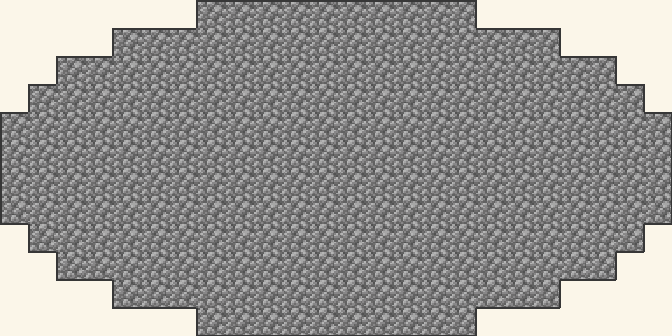
\includegraphics[width=0.45\textwidth]{fig07_2d_ellipse_24x12.png}
\caption{Block Round 上の楕円 $W = 24, H = 12$。長軸方向のセルが短軸方向よりも空けて並ぶことに注目。}
\label{fig:elipse}
\end{figure}

\begin{enumerate}[leftmargin=1.5em,itemsep=0.15em,topsep=0.3em]
  \item 形状を \acc{Ellipse} に切り替え。\emph{Width} と \emph{Height} の2スライダが表示される。
  \item $W = 24$、$H = 12$ に設定。長辺方向の楕円を観察（Figure~\ref{fig:elipse}）。
  \item 討議：「\emph{この形を支配する方程式は $(x/12)^2 + (y/6)^2 = 1$。なぜ $x$ を 12 で、$y$ を 6 で割るのでしょう？}」
\end{enumerate}

\subsection{3D モード、球、楕円体}

\begin{enumerate}[leftmargin=1.5em,itemsep=0.15em,topsep=0.3em]
  \item モードを \acc{3D / Sphere}、サイズ $D = 12$ に。
  \item マウスドラッグで回転。ボクセルで構成された球が現れる。
  \item \emph{Info chip} を表示：体積を記録（「904 blocks = $14 \times 64 + 8$」）。
  \item \acc{Ellipsoid}、$W = 20$、$H = 10$、$D = 12$ に変更。
  \item \emph{Cut} スライダを \texttt{Y} 軸 50\% に（Figure~\ref{fig:cortes}(a) 参照）。上半分が消える。
  \item 対角軸 $\swarrow$/$\nearrow$（45°、Figure~\ref{fig:cortes}(c)）に切替。斜め切断を討議。
\end{enumerate}

\subsection{マインクラフトへの出力}
\begin{enumerate}[leftmargin=1.5em,itemsep=0.15em,topsep=0.3em]
  \item キャンバス端の\emph{ダウンロード}ボタンを示す：PNG。
  \item \emph{Export Schematic} ボタンを示す：\texttt{.schem}（Sponge Schematic v2）を保存。
  \item （可能なら）Litematica 経由でのマインクラフト Java 読込を実演。付録~\ref{ap:litematica} 参照。
\end{enumerate}

% =============================================================================
\newpage
\section{演習問題}\label{ap:exerc}

\textbf{指示：}個人で解答。Block Round で答えを確認してもよいが、\emph{数学的根拠の記述は必須}。手書きまたはタイプ提出可。

\subsection*{問題 1 --- 円の方程式}
\textbf{問題：}原点 $(0, 0)$ を中心とし半径 $r = 7$ の円を考える。次の各点が円の\emph{内部}・\emph{外部}・\emph{周上}のどれにあるか、方程式で根拠を付けて答えよ。
\begin{enumerate}[label=\alph*),leftmargin=1.5em,itemsep=0.1em,topsep=0.2em,nosep]
  \item $(3, 4)$ \hfill \emph{解答：}内部（$9 + 16 = 25 < 49$）。
  \item $(5, 5)$ \hfill \emph{解答：}\acc{外部}（$25 + 25 = 50 > 49$、$\sqrt{50} \approx 7{,}07$ なので）。
  \item $(0, 7)$ \hfill \emph{解答：}周上。
  \item $(-7, 0)$ \hfill \emph{解答：}周上。
\end{enumerate}

\textit{教育的注意：}(b) は意図的な罠である。

\subsection*{問題 2 --- スタックとチェストの算法}
\textbf{問題：}ユークリッド・アルゴリズムで $D = 8$ の球を考える。連続体積 $V = \tfrac{4}{3}\pi \cdot 4^3 \approx 268{,}1$、離散体積 $V_{\mathrm{disc}} = 268$。
\begin{enumerate}[label=\alph*),leftmargin=1.5em,itemsep=0.1em,topsep=0.2em,nosep]
  \item cobblestone のスタックは何個必要か？ $q$ スタック $+$ $r$ 余りブロック の形式で答えよ。
  \item これらをすべて格納するのにシングルチェスト（27 スロット）は何個必要か？
  \item サバイバルモードで、鉄製つるはしで 0,5秒に1ブロック採掘できるとして、総採掘時間は？
\end{enumerate}

\emph{解答：}(a) $268 = 4 \times 64 + 12$、すなわち \acc{4 スタック満杯 $+$ 12 余りブロック}（インベントリで5スロット使用）。(b) シングルチェスト1個で十分（27スロット中5スロットしか使わない）。(c) $268 \times 0{,}5 = 134$ 秒 $\approx$ 2分14秒。

\subsection*{問題 3 --- $D=20$ における3アルゴリズム比較}
\textbf{問題：}Block Round で $D = 20$ の円を三つのアルゴリズムで生成。
\begin{enumerate}[label=\alph*),leftmargin=1.5em,itemsep=0.1em,topsep=0.2em,nosep]
  \item 各アルゴリズムの面積（ブロック数）を記録せよ。
  \item 材料を最小化するのはどれ？最大化するのはどれ？
  \item 最大値と最小値の差を\emph{スタック}換算すると？節約のために小さい方を選ぶ価値はあるか？
\end{enumerate}

\emph{想定解答：}ユークリッド $\approx 316$ ブロック（4スタック $+$ 60余り）、ブレゼンハム $\approx 316$、閾値 $\approx 332$ ブロック（5スタック $+$ 12余り）。差：$\approx 1$ スタック。大型プロジェクト（$D \geq 32$）では蓄積する。

\subsection*{問題 4 --- ドームの体積と倉庫計画}
\textbf{問題：}$D = 16$、ユークリッド、Y軸50\% 切断のドームを考える。
\begin{enumerate}[label=\alph*),leftmargin=1.5em,itemsep=0.1em,topsep=0.2em,nosep]
  \item 球全体の連続体積。
  \item ドーム（上半分）の体積。
  \item ドームのブロックすべてを格納するのにラージチェストは何個必要か？
  \item ドームの下に $16 \times 16$ の床を1層敷くだけのブロック余りはあるか？
\end{enumerate}

\emph{解答：}
(a) $V = \tfrac{4}{3}\pi \cdot 8^3 \approx 2\,144{,}66$、$V_{\mathrm{disc}} \approx 2\,145$。(b) $V_{\mathrm{dome}} \approx 1\,095$。(c) $\lceil 1\,095 / 3\,456 \rceil = 1$ ラージチェスト。(d) 余り：$3\,456 - 1\,095 = 2\,361$ ブロック。床 $16 \times 16 = 256$ ブロック。残りは 2\,105 ブロックで、床ともう1層のベンチを建てられる。

\subsection*{問題 5 --- 「巨大円卓」型楕円体}
\textbf{問題：}$W = 24$、$H = 8$、$D = 24$ の楕円体（「卓子」のような扁平形状）を考える。
\begin{enumerate}[label=\alph*),leftmargin=1.5em,itemsep=0.1em,topsep=0.2em,nosep]
  \item 連続体積。
  \item Block Round で見積もる離散体積。
  \item Oak Planks のラージチェスト3個を購入した場合、余るか足りないか？
\end{enumerate}

\emph{解答：}
(a) $V = \tfrac{4}{3}\pi \cdot 12 \cdot 4 \cdot 12 \approx 2\,413$。
(b) $V_{\mathrm{disc}} \approx 2\,400$（アルゴリズムにより $\pm 10$ 変動）。
(c) 購入容量：$3 \times 3\,456 = 10\,368$ ブロック。\emph{大幅に余る}---$\approx 8\,000$ ブロック余剰。\emph{過剰な購入である}。理想はラージチェスト1個（$\approx 1\,000$ ブロック余り）。

\subsection*{問題 6 --- WorldEdit 対 Block Round}
\textbf{問題：}WorldEdit のコマンド \cmd{//sphere stone 15} はブレゼンハム 3D に似たアルゴリズムを使用。Block Round のブレゼンハム・$D = 30$ の出力と比較せよ。
\begin{enumerate}[label=\alph*),leftmargin=1.5em,itemsep=0.1em,topsep=0.2em,nosep]
  \item 両者は完全に同一であるべきか？
  \item 同一でないとしたら、その理由は？最低2つ挙げよ。
\end{enumerate}

\emph{解答：}
(a) \emph{ほぼ一致する}---どちらもブレゼンハム3D。(b) 相違の理由：(i) 実装言語が異なる（Block Round は JavaScript、WorldEdit は Java）；(ii) 直径の偶奇の扱い（偶数 vs 奇数）；(iii) 経験的閾値の存在（どちらかが内部的に閾値を使う場合）。典型的な差：$D = 30$ で 0--6 ブロック。

\subsection*{問題 7 --- 八面体対称性による建築}
\textbf{問題：}マインクラフトで中心 $(0, 72, 0)$ の球 $D = 16$ を対称性で建てる計画。1オクタント（$+x, +y, +z$、$\approx 268$ ブロック）を建て、\cmd{/clone} で7回鏡映する。
\begin{enumerate}[label=\alph*),leftmargin=1.5em,itemsep=0.1em,topsep=0.2em,nosep]
  \item 7つの \cmd{/clone} コマンドを書け（地形を消さないよう \cmd{mode:masked} を使うこと）。
  \item オクタント手動建築 + コマンドの推定総時間。
\end{enumerate}

\emph{解答：}

\begin{minecraft}[コマンド列]
\cmd{/clone 0 72 0 7 79 7 -8 72 0 mode:masked} \quad （$-x$ 鏡映）\\
\cmd{/clone 0 72 0 7 79 7 0 64 0 mode:masked} \quad\quad （$-y$ 鏡映）\\
\cmd{/clone 0 72 0 7 79 7 0 72 -8 mode:masked} \quad （$-z$ 鏡映）\\
\cmd{/clone -8 72 0 -1 79 7 mode:masked} \quad\quad\;\; （$-x,-y$ オクタント）\\
\cmd{/clone 0 64 -8 7 71 -1 mode:masked} \quad\quad\;\; （$-y,-z$ オクタント）\\
\cmd{/clone -8 72 -8 -1 79 -1 mode:masked} \quad\;\; （$-x,-z$ オクタント）\\
\cmd{/clone -8 64 -8 -1 71 -1 mode:masked} \quad\;\; （$-x,-y,-z$ オクタント）
\end{minecraft}

時間：$\sim$ 5 分（手動オクタント、サバイバル）+ $\sim$ 3 秒（7クローン）。

\subsection*{問題 8 --- 最終プロジェクト}
\textbf{問題：}グループ制作物（活動~\ref{at:53}）の完成後、次に答えよ。
\begin{enumerate}[label=(\arabic*),leftmargin=1.7em,itemsep=0.15em,topsep=0.2em,nosep]
  \item 使用した幾何図形（円・楕円・球・楕円体）とそのパラメータ（直径または半軸）をリスト化せよ。
  \item 主要図形について、選んだアルゴリズムは？理由は？他の2つでは得られない視覚効果は何か？
  \item 3D 切断はあったか？あった場合、そのうち\emph{一つ}を数学的に不等式として記述せよ。
  \item マインクラフトのサバイバルで実際に建てるとしたら、スタック・ラージチェストは何個必要か？
  \item 作品は何らかの日本の文化的参照（縄文土器、古墳、伝統幾何文様、和算、安藤忠雄・隈研吾・SANAA の現代建築、マインクラフト日本コミュニティ）と対話しているか？コメントせよ。
\end{enumerate}

% =============================================================================
\newpage
\section{情報科教室のない学校のための適応}\label{ap:adapt-analog}

本適応は、コンピュータへのアクセスが不可能な場合（離島・過疎地、災害復興地、定時制夜間の一部などで起こりうる）にシーケンスを\emph{完全に紙で}実施可能にする。概念的軸は維持され、物的支持のみが変わる。

\subsection{各授業の代替案}

\begin{center}
\small
\begin{tabularx}{\textwidth}{@{}p{0.13\textwidth}p{0.32\textwidth}X@{}}
\toprule
\textbf{授業} & \textbf{原案の活動} & \textbf{アナログ適応} \\
\midrule
1 & Block Round の実演（1.3） & 教員が黒板大の事前印刷格子の上に、3つのアルゴリズムによる $D = 10$ 円を手描き---1つずつ別図。Figure~\ref{fig:comp-d10}、Figure~\ref{fig:comp-d20} を参考に印刷可能。 \\
\addlinespace[3pt]
2 & ソフトでの定量比較（\ref{at:25}） & 三つの $D = 16$ 円を事前描画したシートを配布し、手作業で計数。 \\
\addlinespace[3pt]
3 & 3D 球の生成（\ref{at:31}, \ref{at:32}） & 球の\emph{スライス}（$z = 0, 1, 2, \ldots$）を方眼紙に印刷して配布。生徒は積層で立体心象を構築。各シートがマインクラフトの\emph{1層}のブロックを模擬。 \\
\addlinespace[3pt]
4 & マインクラフト・コマンド（\ref{at:42}） & コマンドを日本語の\emph{建築指示文}に置換。生徒は方眼紙の上で実行を模擬。 \\
\addlinespace[3pt]
5 & マインクラフトでの実建築（\ref{at:53}） & \emph{レゴ}（利用可能なら）、色鉛筆（草色・土茶色）で着色した方眼紙、または芸術科で生徒が折った\emph{紙のキューブ}による構築。 \\
\bottomrule
\end{tabularx}
\end{center}

\subsection{補助シート}
完全アナログ版のために事前準備を推奨する資料：
\begin{itemize}[leftmargin=1.3em,itemsep=0.1em,topsep=0.2em,nosep]
  \item A3 用紙に定規で描いた $30 \times 30$ の格子1枚。
  \item 生徒1人に5mm 方眼紙 5 枚（A4）のセット。
  \item 三つの比較円を事前印刷した1枚---Figure~\ref{fig:comp-d10}、Figure~\ref{fig:comp-d20} を A4 サイズで。
  \item 第5授業のアナログ版のため：グループあたり 8 個の\emph{紙のキューブ}を事前に折る（cobblestone、oak、quartz、diamond のテクスチャを紙に印刷して貼る）。
\end{itemize}

\subsection{地域の伝統知の活用}
強い工芸伝統を持つ地域の学校（沖縄の織物・首里織、京都の西陣織、加賀友禅、八重山ミンサー、アイヌのアットゥシ、福島の会津漆器、佐賀の有田焼など）では、第3授業を地域の\emph{伝統工芸の担い手や職人}の訪問講話で\emph{豊かにできる}。織師、染師、陶芸家、漆芸家、和紙職人が、自分の言語で円や対称をどう「ラスタライズ」しているかを示す。この接近は、本シーケンスの民族数学的方向性を実現し、文部科学省「外国人児童生徒等教育の充実方策について」（平成28年）の趣旨にも沿う。

% =============================================================================
\newpage
\section{教員のための専門用語集}\label{ap:glos}

\begin{itemize}[leftmargin=1.4em,itemsep=0.3em,topsep=0.3em]
  \item \acc{アルゴリズム} --- 問題を解くための有限かつ明確に定義された命令の列。Block Round の三アルゴリズム（Figure~\ref{fig:comp-d10}）は同じ問題に対する異なる手続き。
  \item \acc{Bresenham のアルゴリズム} --- 1965年、Jack Bresenham（IBM）が発表。元は直線用、後に Pitteway、Kappel らが楕円に拡張。\emph{整数演算のみ}を用いるのが特徴。活動~\ref{at:23} 参照。
  \item \acc{シングルチェスト} --- マインクラフトの容器、27 スロット。容量：$27 \times 64 = 1\,728$ 個。
  \item \acc{ラージチェスト} --- 隣接した2つのチェストが結合して54スロットの容器となる。容量：$54 \times 64 = 3\,456$ 個。
  \item \acc{ブロック} --- マインクラフトの建造単位。$1\times1\times1$ の立方体、6面にテクスチャ。数学用語では\emph{ボクセル}。
  \item \acc{Canvas} --- ブラウザ内の HTML 要素、2D/3D 描画空間を提供。
  \item \acc{\code{/clone}} --- マインクラフトのバニラコマンド、矩形領域を別位置にコピー。構文：\cmd{/clone x1 y1 z1 x2 y2 z2 dx dy dz}。対称性建築に不可欠。
  \item \acc{共通テスト} --- 大学入学共通テスト（令和3年度〜、旧センター試験）。
  \item \acc{陰関数方程式} --- $F(x, y) = 0$ の形式の方程式。楕円の例：$(x/r_x)^2 + (y/r_y)^2 - 1 = 0$。
  \item \acc{民族数学（エスノマスマティクス）} --- ブラジルの Ubiratan D'Ambrosio が体系化した研究領域。
  \item \acc{\code{/fill}} --- マインクラフトのバニラコマンド、矩形ボックスを単一ブロックで埋める。構文：\cmd{/fill x1 y1 z1 x2 y2 z2 minecraft:stone}。
  \item \acc{GIGAスクール構想} --- 文部科学省が2019年〜推進する1人1台端末整備事業。
  \item \acc{高専} --- 高等専門学校（5年制）。
  \item \acc{情報I/情報II} --- 高等学校情報科の必修科目（令和4年度実施）と発展科目（令和5年度開講）。
  \item \acc{JMO} --- 日本数学オリンピック。
  \item \acc{JOI} --- 日本情報オリンピック。
  \item \acc{APPI} --- 個人情報保護法（個人情報の保護に関する法律、平成15年制定）。
  \item \acc{Litematica} --- マインクラフト Java版の代表的 mod、スキマティックを読み込んで建築の半透明\emph{ゴースト}を表示する。無料。
  \item \acc{マインクラフト教育版} --- マインクラフトの教育用エディション。Microsoft 365 Education ライセンスで学校に無償提供。
  \item \acc{RIMS} --- 京都大学数理解析研究所。
  \item \acc{パック／スタック} --- マインクラフトのインベントリ1スロット内に最大64個の同一ブロック。
  \item \acc{ピクセル} --- \emph{picture element} の略。2Dの場合。
  \item \acc{PWA} --- \emph{Progressive Web App}。インストール可能、オフライン動作可能な Web アプリ。
  \item \acc{ラスタライゼーション} --- 連続的な幾何記述を pixel（2D）または voxel（3D）の行列に変換する処理。
  \item \acc{Schematica} --- Litematica の代替 mod、類似機能。
  \item \acc{Schematic（\texttt{.schem}）} --- マインクラフトの領域を直列化するファイル形式（Sponge Schematic v2、gzip + NBT）。
  \item \acc{半軸} --- 楕円で、中心から軸方向の端点までの距離。
  \item \acc{SSH} --- スーパーサイエンスハイスクール（文部科学省指定校）。
  \item \acc{\code{//sphere}} --- WorldEdit のコマンド、球を構築。構文：\cmd{//sphere <block> <radius>}。
  \item \acc{スロット} --- マインクラフトのインベントリの単位セル。プレイヤーの全インベントリ：36 スロット（$9 \times 4$）。
  \item \acc{ボクセル} --- \emph{volume element} の略。pixel の3D版。マインクラフトでは各\emph{ブロック}が1ボクセル。
  \item \acc{WebGL} --- ブラウザでの3Dグラフィック・プログラミング用ライブラリ。
  \item \acc{WorldEdit} --- マインクラフト Java版の超人気 mod、大規模建築用の上級コマンド（\cmd{//sphere}、\cmd{//hsphere}、\cmd{//ellipsoid}、\cmd{//cyl}、\cmd{//schem load}）を追加する。
  \item \acc{和算} --- 江戸時代の日本独自の数学（関孝和・建部賢弘ら）。
  \item \acc{学習指導要領} --- 文部科学省が告示する全国共通カリキュラム（10年ごとに改訂、直近は平成30年告示・令和4年実施）。
\end{itemize}

% =============================================================================
\newpage
\section{チュートリアル：Block Round から Litematica 経由でマインクラフトへ}\label{ap:litematica}

本付録は、Block Round からの出力をマインクラフト Java版に \emph{Litematica} mod で読み込む完全なフローを記述する。所要時間（初回）：15分。

\subsection{前提条件}
\begin{itemize}[leftmargin=1.3em,itemsep=0.1em,topsep=0.2em,nosep]
  \item マインクラフト Java版（\emph{Mojang Store} で購入；無料の\emph{マインクラフト教育版}も調整次第で利用可能）。
  \item 使用するマインクラフトのバージョンに対応する\emph{Fabric Loader}（通常は最新版：\url{https://fabricmc.net/use/}）。
  \item Mods：\emph{Fabric API} と \emph{Litematica}（\url{https://www.curseforge.com/minecraft/mc-mods/litematica}）。
  \item ブラウザで Block Round を開いた状態。目的の図形は作成済み。
\end{itemize}

\subsection{ステップ1：Block Round から出力}
\begin{enumerate}[leftmargin=1.5em,itemsep=0.15em,topsep=0.3em]
  \item Block Round で目的の図形を設定（モード、形状、直径、アルゴリズム、ブロック、切断）。\emph{Info chip} で体積を確認。
  \item キャンバス右上の\emph{Export Schematic}ボタン（2番目のアイコン）をクリック。\texttt{.schem} ファイルがダウンロードされる。
\end{enumerate}

\subsection{ステップ2：Litematica の導入}
\begin{enumerate}[leftmargin=1.5em,itemsep=0.15em,topsep=0.3em]
  \item 使用するマインクラフトのバージョンに対応する Fabric Loader をインストール。
  \item 同バージョン対応の\emph{Fabric API}と\emph{Litematica}をダウンロード。両方を \texttt{.minecraft/mods/} に置く。
  \item プロファイル \emph{fabric-loader-x.y.z-1.20.x} でマインクラフトを起動。
\end{enumerate}

\subsection{ステップ3：スキマティックの読込}
\begin{enumerate}[leftmargin=1.5em,itemsep=0.15em,topsep=0.3em]
  \item \texttt{.schem} ファイルを \texttt{.minecraft/schematics/} に置く（または Litematica 設定で指定したフォルダに）。
  \item ワールド内（クリエイティブまたはサバイバル）で、キー \texttt{M} で Litematica メニューを開く。
  \item \emph{Load Schematic} $\rightarrow$ ファイルを選択 $\rightarrow$ \emph{Load} をクリック。
  \item リストにスキマティックが表示される。それを選んで \emph{Placement}：半透明な\emph{ゴースト}がワールドに現れる。
  \item 移動コントロール（\texttt{M} $\rightarrow$ \emph{Placements}）でゴーストを目的位置に移動。平地ならボックス下隅 $(x_1, y_1, z_1)$ を地面に合わせるだけ。
\end{enumerate}

\subsection{ステップ4：建築}
\begin{enumerate}[leftmargin=1.5em,itemsep=0.15em,topsep=0.3em]
  \item \emph{クリエイティブ}：ゴースト上を飛行しブロックを置く。Litematica が正しいブロックは緑、誤りは赤で表示する。直径12の球は約5分。
  \item \emph{サバイバル}：手順は同じだが、事前にブロック収集が必要。活動~\ref{at:41} のスタック・ラージチェスト計算を用いて準備する。
  \item 代替案：WorldEdit のあるサーバーなら、\cmd{//schem load <filename>} に続いて \cmd{//paste -a} で瞬時建築。
\end{enumerate}

\subsection{ステップ5：検証}
Litematica は欠落・誤種別・誤位置のブロックを赤で表示する。\texttt{Z} キーでゴーストの可視・不可視を切り替えて実建築と比較できる。

\subsection{よくあるトラブルシューティング}
\begin{itemize}[leftmargin=1.3em,itemsep=0.15em,topsep=0.3em,nosep]
  \item \emph{スキマティックがリストに出ない：}ファイルが正しいフォルダにあるか、Litematica のバージョンがマインクラフト本体と互換かを確認。
  \item \emph{ブロックが灰色／違うブロックになる：}Block Round の出力に含まれるブロック名が、使っているマインクラフト・バージョンに存在しない可能性。テキストエディタでスキマティックを開いて名前を確認。
  \item \emph{ゴーストが浮く：}Placement メニューの \emph{Rotation/Mirror} で位置調整。球なら回転は無関係。楕円なら回転を合わせる。
\end{itemize}

\vspace{2em}
\begin{center}
\color{muted}\small\sffamily
--- 授業計画 完 ---
\end{center}

\end{document}
